\cleardoublepage

\chapter{Image Processing}
\label{ch:initial_work}

\par This chapter aims at discussing how the image processing stage was built.
\par Initially in section \ref{sec:testruns} a performance comparison between some state-of-the-art image recognition algorithms and object detection models was done. Section \ref{sec:alpha_retrieval} describes a very raw first attempt at an image retrieval system using only object detection. Subsequently in section \ref{sec:scene_recognition} it is demonstrated how the scene recognition algorithm worked. Finally section \ref{sec:process_dataset} clarifies how all of the images in the imageclef dataset were processed.



  \section{Test Runs}
  \label{sec:testruns}

   With the goal of comparing the different image recognition algorithms and object detection models a few test runs were made. The models and algorithms were provided trough a computer vision python library called imageAI, which allows the ability to easily use state-of-the-art AI features. It supports algorithms for image prediction, custom image prediction, object detection, video detection, video object tracking and image predictions trainings \cite{ImageAI}.

  The test runs consist on feeding each of the models and algorithms with one picture manually chosen beforehand. Each model produces predictions on what the image represents or what the objected detected is. The prediction probability ranges in an interval between [0,100]. This prediction probability represents the certainty of the model or algorithm in the respective prediction.


  \par Sections \ref{sec:image_test} and \ref{sec:object_test} provide examples of the performance test runs done to the models and algorithms.

  \subsection{Image Recognition test runs}
  \label{sec:image_test}


  The imageAI library allows the usage of 4 image recognition algorithms for image recognition which are DenseNet, inceptionV3, ResNet50, and SquezeeNet.

  The next page shows three examples of some test runs done to these algorithms. The examples are exhibited in the following way : on the left a  picture to be analysed is present and on the right the respective graph with the results is displayed. The graphs are structured in the following manner : the X axis represents the predictions, the Y axis represents the percentage probability certainty for the respective prediction and the color represents the algorithm used.

  The obtained results are discussed in section \ref{sec:results_image}





\newpage



    \begin{figure}[H]
      \centering
      \captionsetup{justification=centering}
      \begin{subfigure}{0.25\textwidth}
      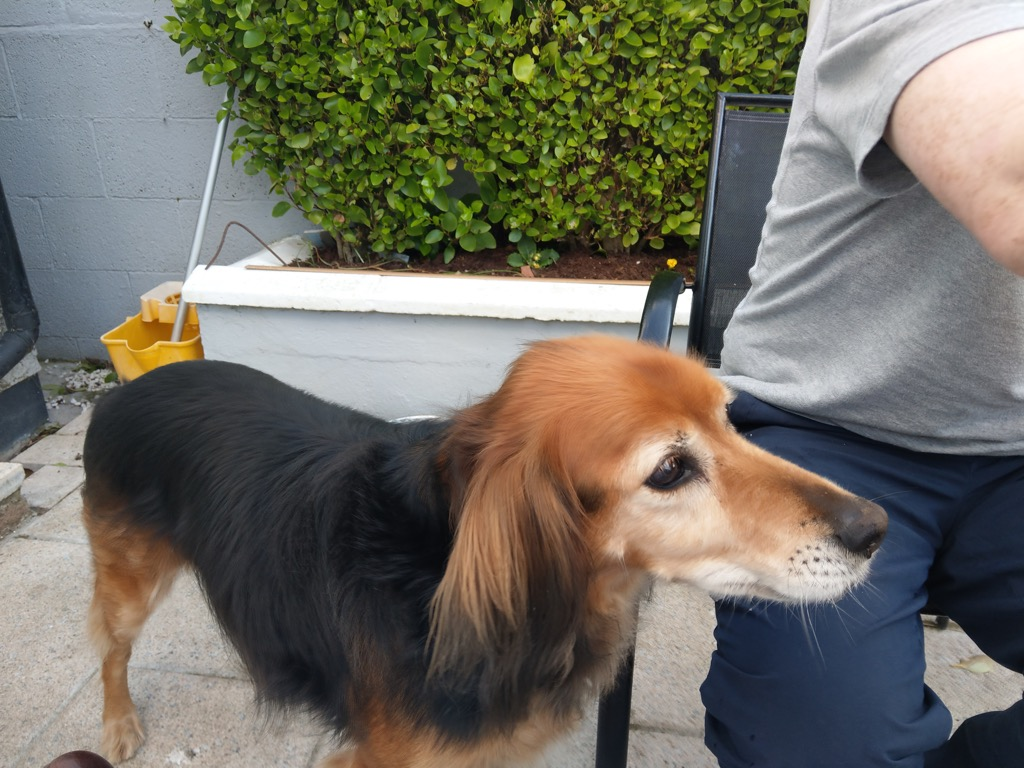
\includegraphics[width=\textwidth]{Sections/4InitialWork/4_images/run1_pic.jpg} 
      \end{subfigure}
      \begin{subfigure}{0.74\textwidth}
      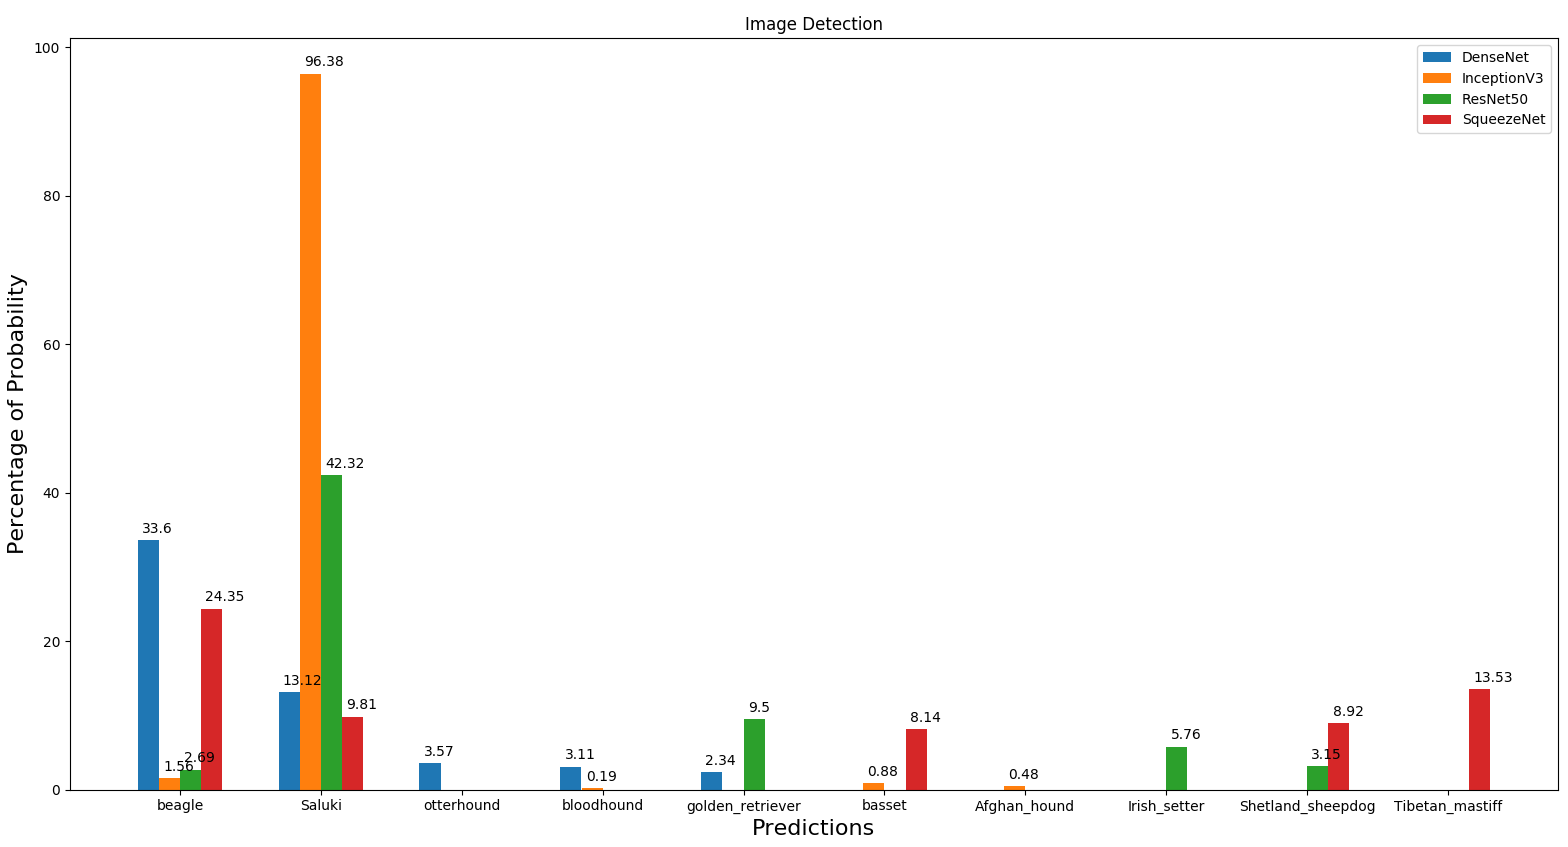
\includegraphics[width=\textwidth]{Sections/4InitialWork/4_images/run1_res.png}
      \end{subfigure}
      \centering
      \captionsetup{justification=centering}
      \begin{subfigure}{0.25\textwidth}
      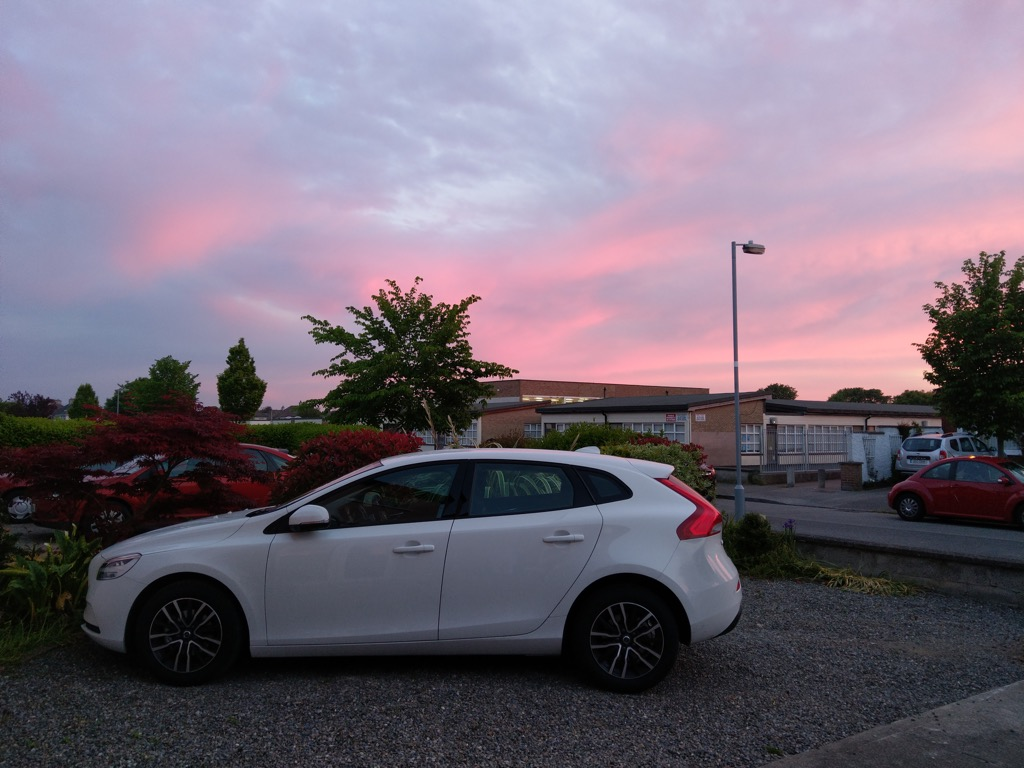
\includegraphics[width=\textwidth]{Sections/4InitialWork/4_images/run3_pic.jpg} 
      \end{subfigure}
      \begin{subfigure}{0.74\textwidth}
      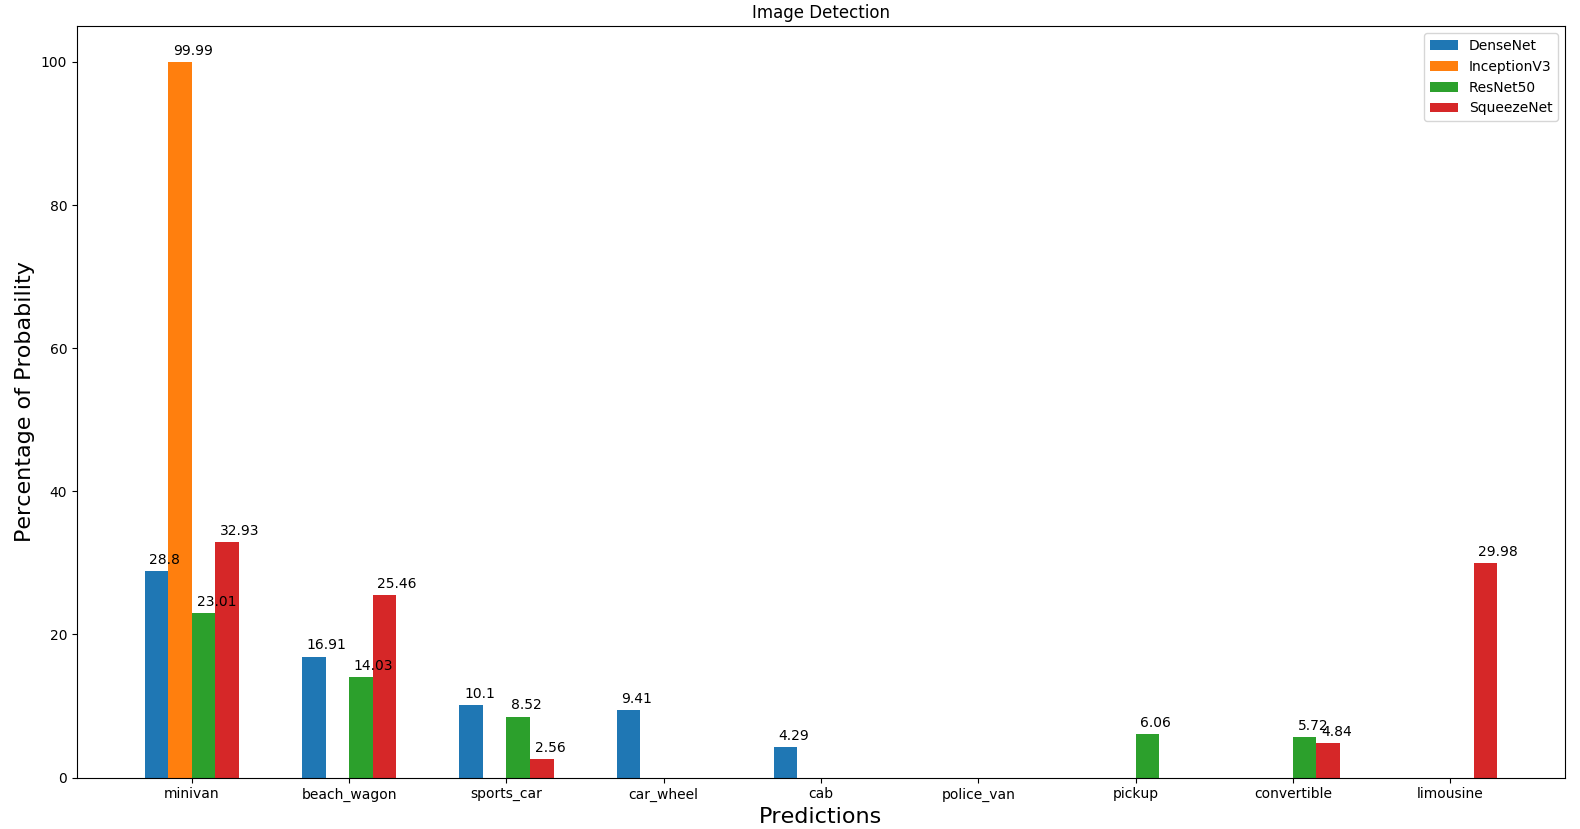
\includegraphics[width=\textwidth]{Sections/4InitialWork/4_images/run3_res.png}
      \end{subfigure}
      \centering
      \captionsetup{justification=centering}
      \begin{subfigure}{0.25\textwidth}
      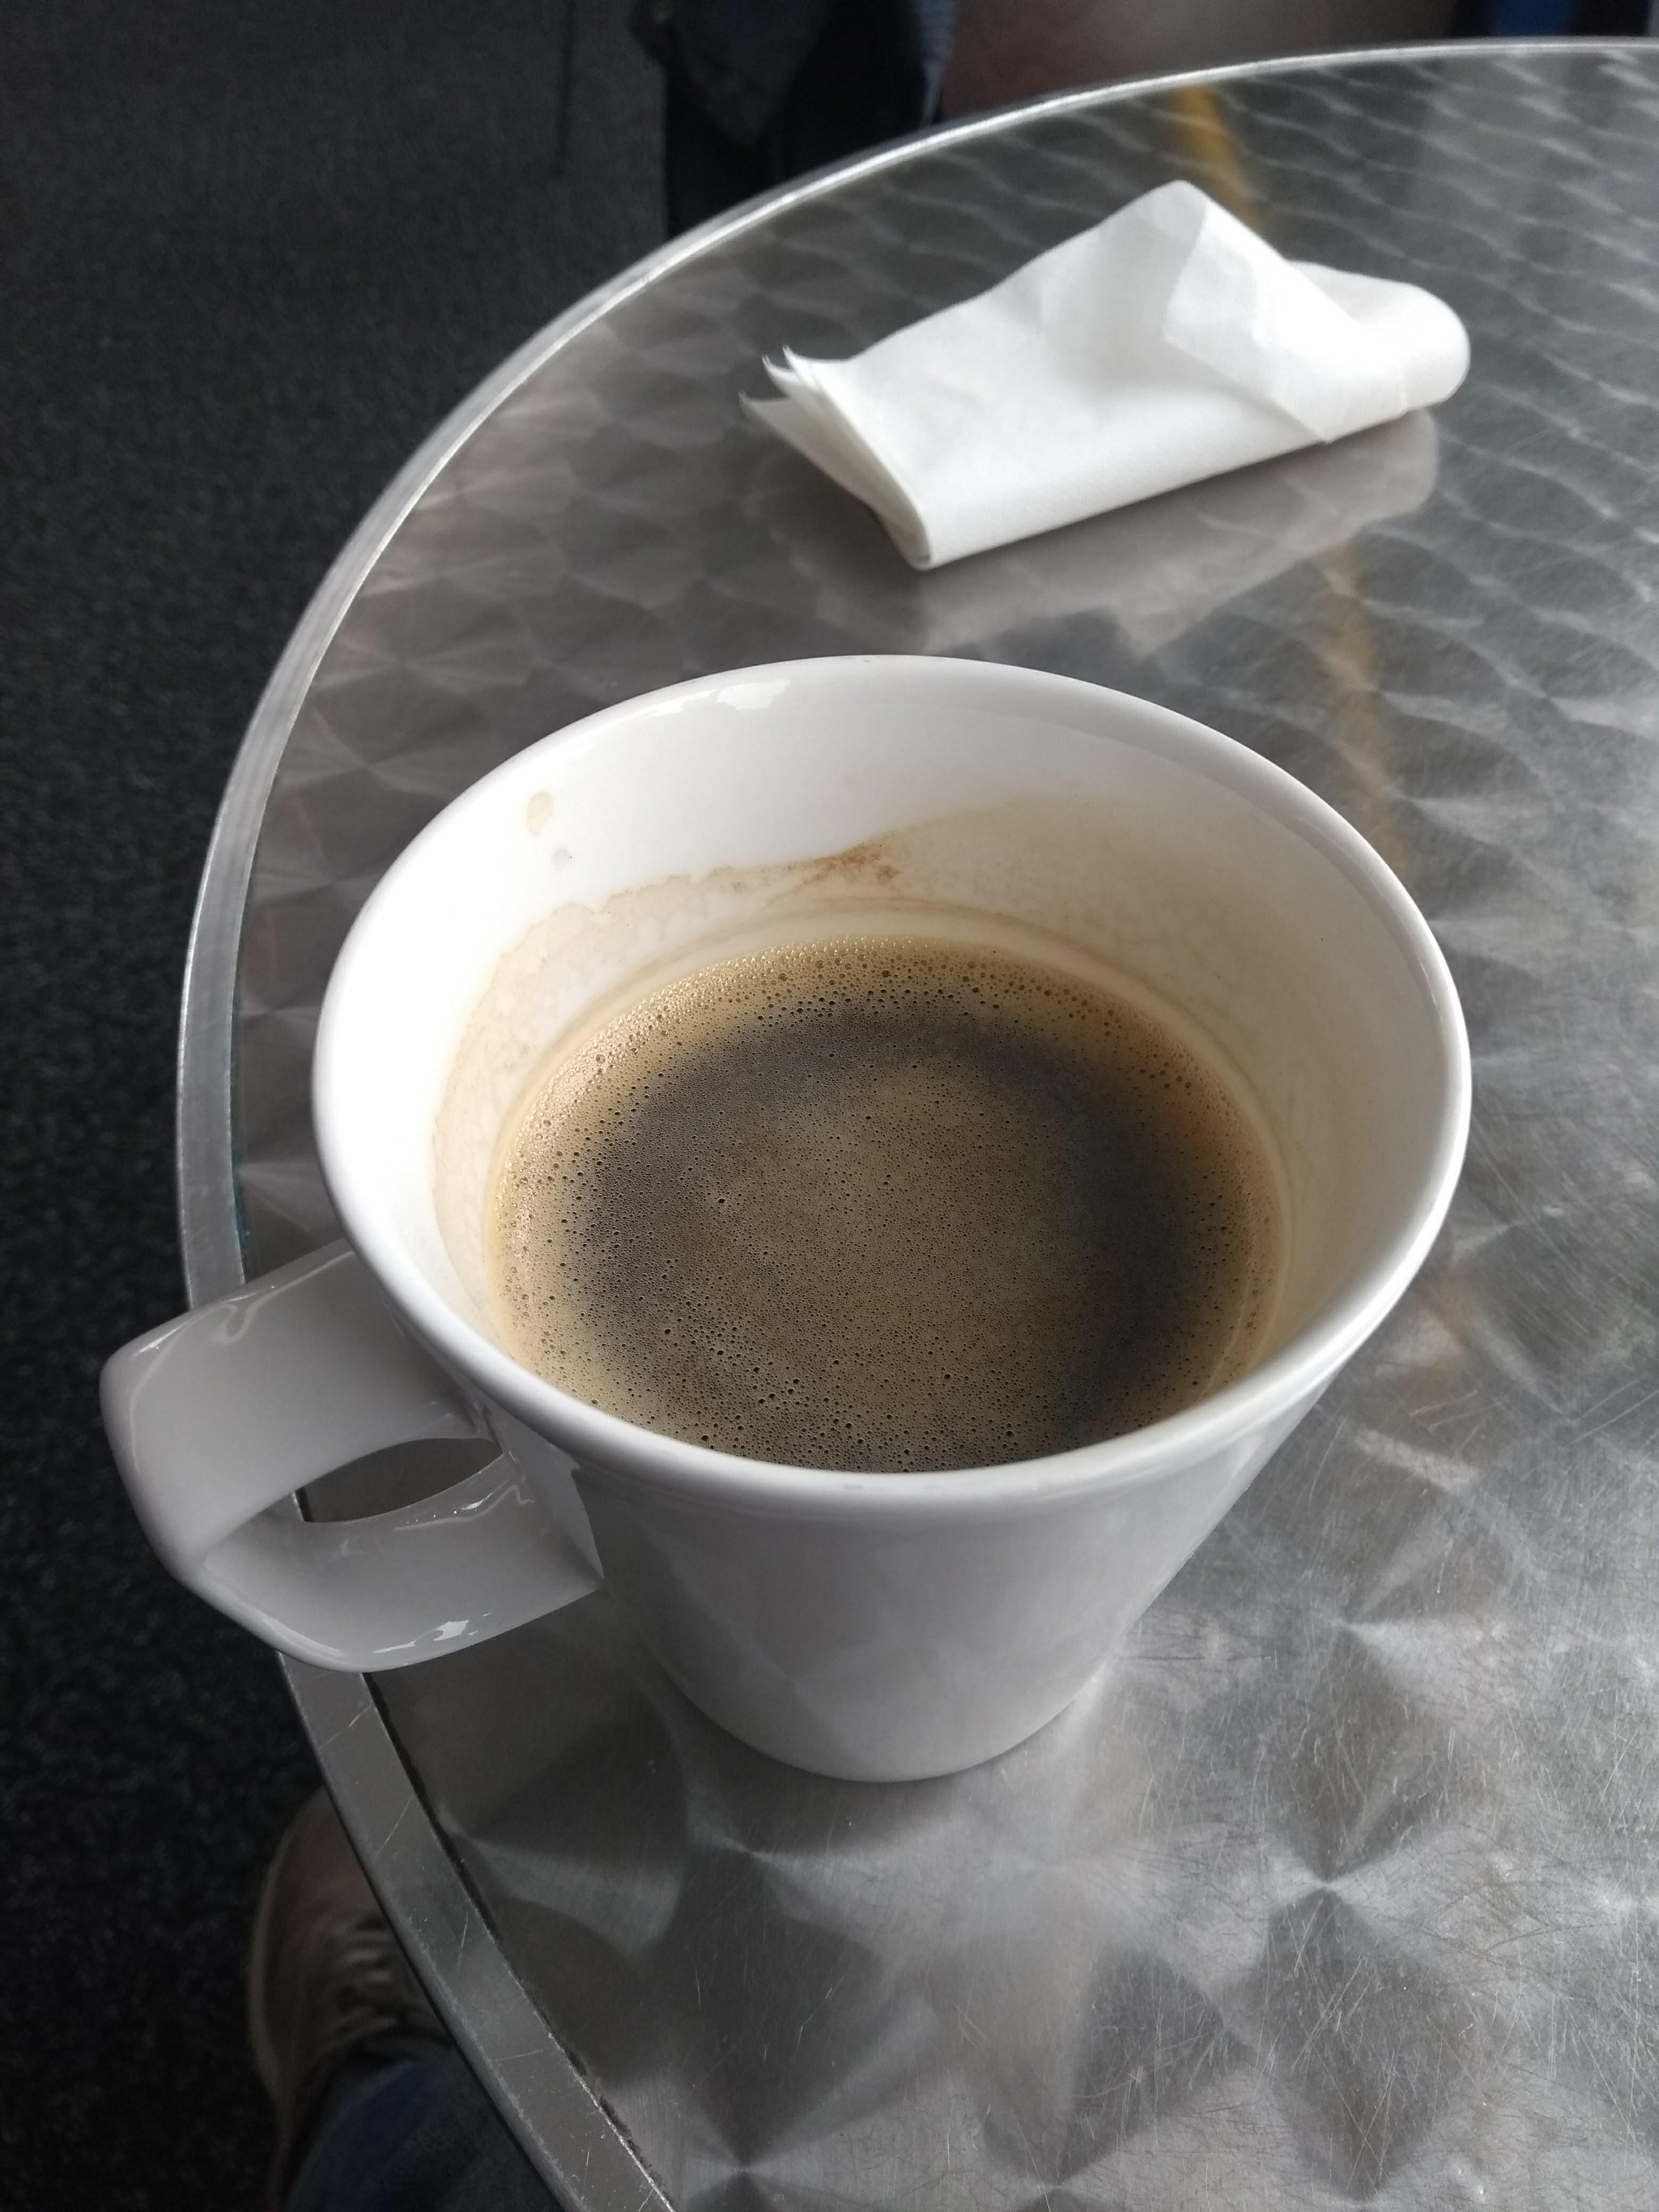
\includegraphics[width=\textwidth]{Sections/4InitialWork/4_images/run4_pic.jpg} 
      \end{subfigure}
      \begin{subfigure}{0.74\textwidth}
      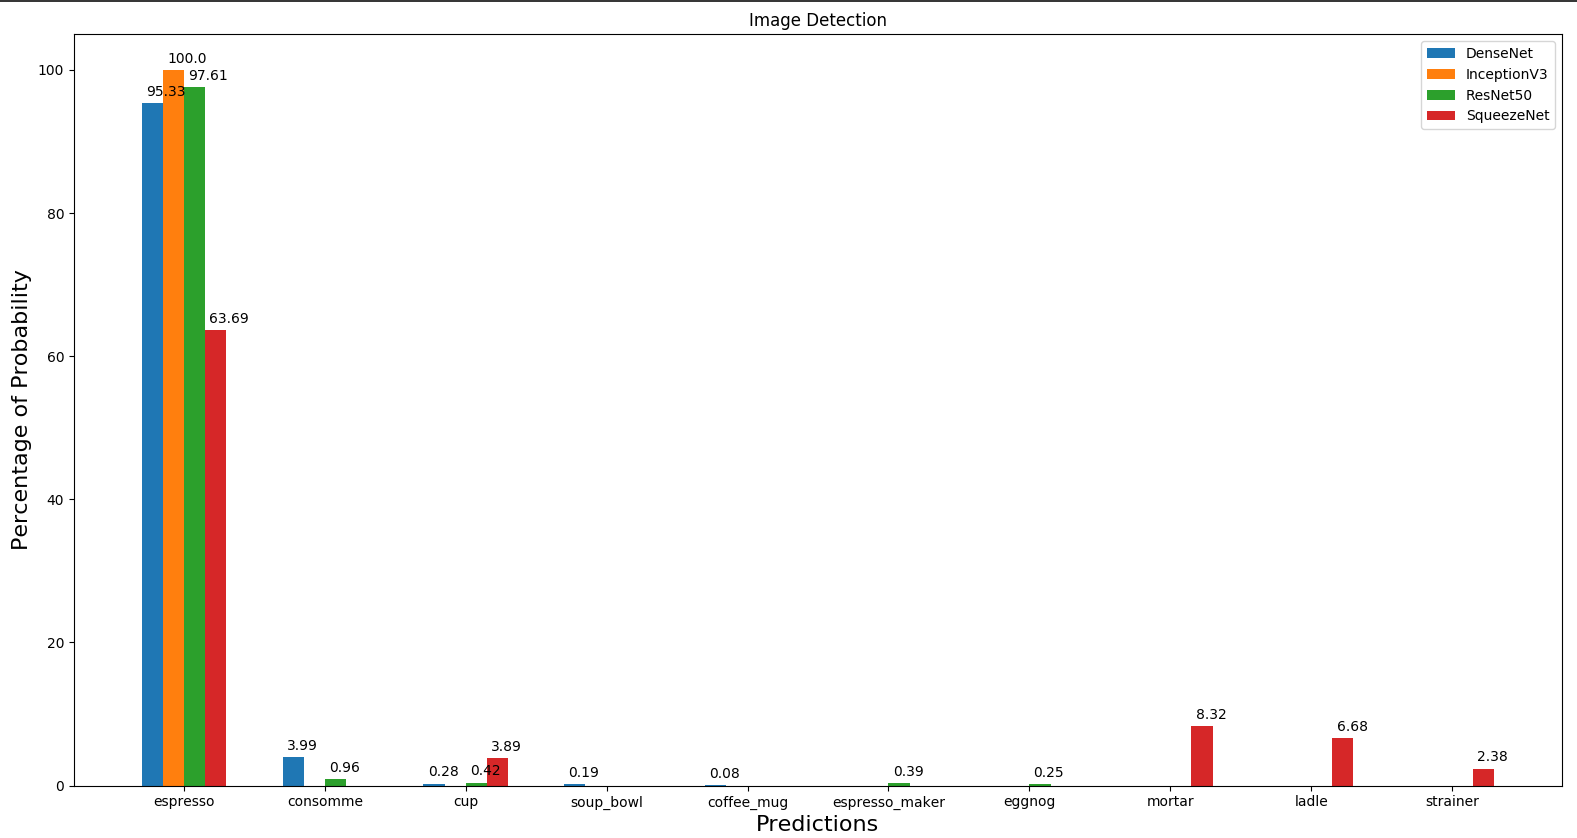
\includegraphics[width=\textwidth]{Sections/4InitialWork/4_images/run4_res.png}
      \end{subfigure}
      
      \caption{Image recognition test runs.}
      \end{figure}


\newpage

\subsubsection{Image Recognition Test Runs Results Analysis}
\label{sec:results_image}


In the first example a picture of a dog (breed Saluki) is analysed. InceptionV3 is the best performer in the first run, predicting correctly with an efficiency of 96.38\% and out performing the other 3 neural networks by a large margin, being that the second best is the ResNet50 with an efficiency of 42.32\%.

For the second example a picture of a car was processed. InceptionV3 predicted with a 99.99\% that the car was a minivan. The shown car is not a minivan but its similar to one, so it is possible to assume that the prediction is correct.

The final example a picture of an espresso coffee is analysed. In this example all image recognition algorithms predicted correctly that the image represents an espresso. However, SquezeeNet only achieved 63.88\% efficiency while InceptionV3 predicted with 100.0\% efficiency.

From the 3 examples that were shown, it is clear that the inceptionV3 algorithm achieved the best results and out performed the other algorithms.






  %%%%%%%%%%%%%%%%%%%%%%%%%%%%%%%%%%%%% OBJECT RECOGNITION   %%%%%%%%%%%%%%%%%%%%%%%%%%%%%%%%%%%%%

  \subsection{Object Detection test runs}
  \label{sec:object_test}

  \par ImageAI provides 3 different models trained on the COCO dataset for object detection that are able to identify up to 80 of the most common objects in everyday life. The models that are provided include RetinaNet, YOLOv3 and TinyYOLOv3. \cite{ImageAI}.

  \par The obtained results are discussed in section \ref{sec:results_objet}


  The objects that these models are able to detect can be seen in the following image : 





    \begin{figure}[htb]
      \centering
      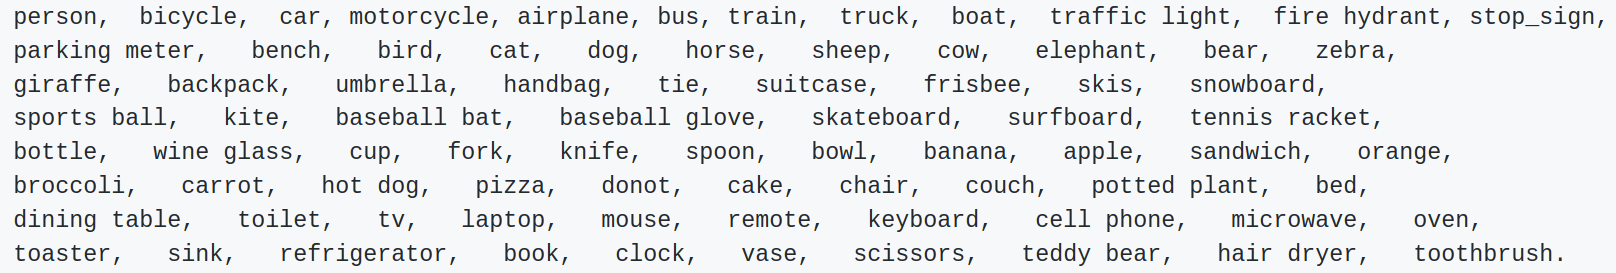
\includegraphics[width = \textwidth]{Sections/4InitialWork/4_images_random/detections.png}
      \caption{Available labels for detection. }
      \label{fig:yolov3} 
  \end{figure}


The following pictures were used to test the described models.


\begin{figure}[H]
  \centering
  \captionsetup{justification=centering}

  \begin{subfigure}{0.3\textwidth}
  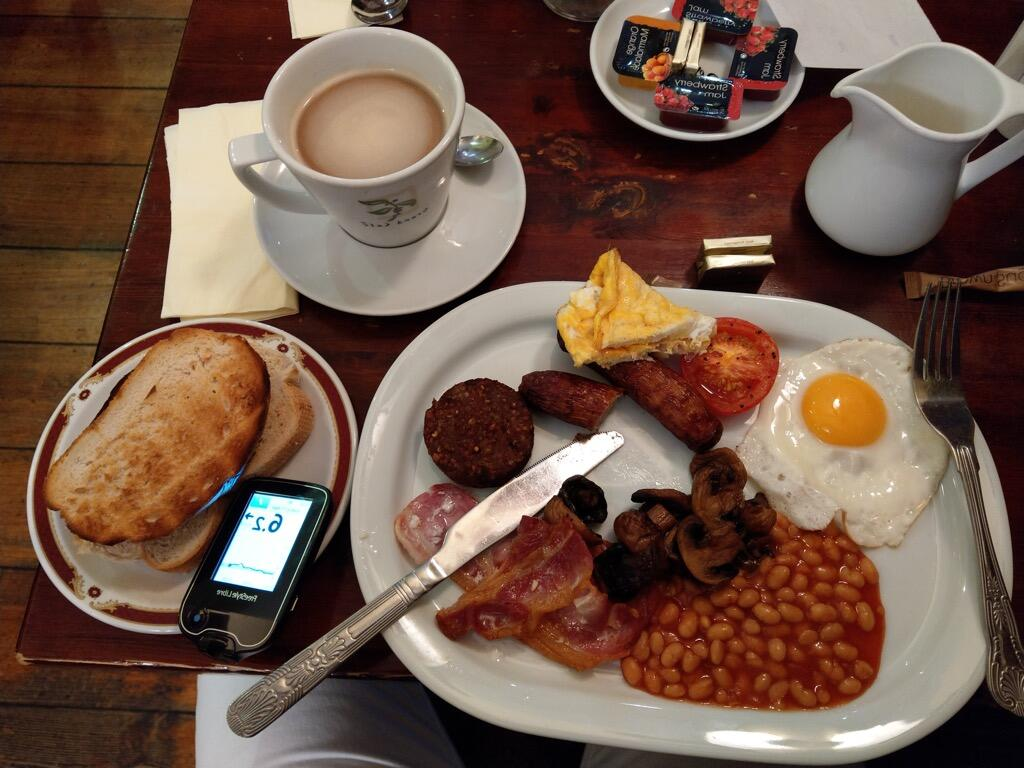
\includegraphics[width=\textwidth]{Sections/4InitialWork/4_images_obj_run1/photo.jpg} 
  \end{subfigure}
  \begin{subfigure}{0.3\textwidth}
  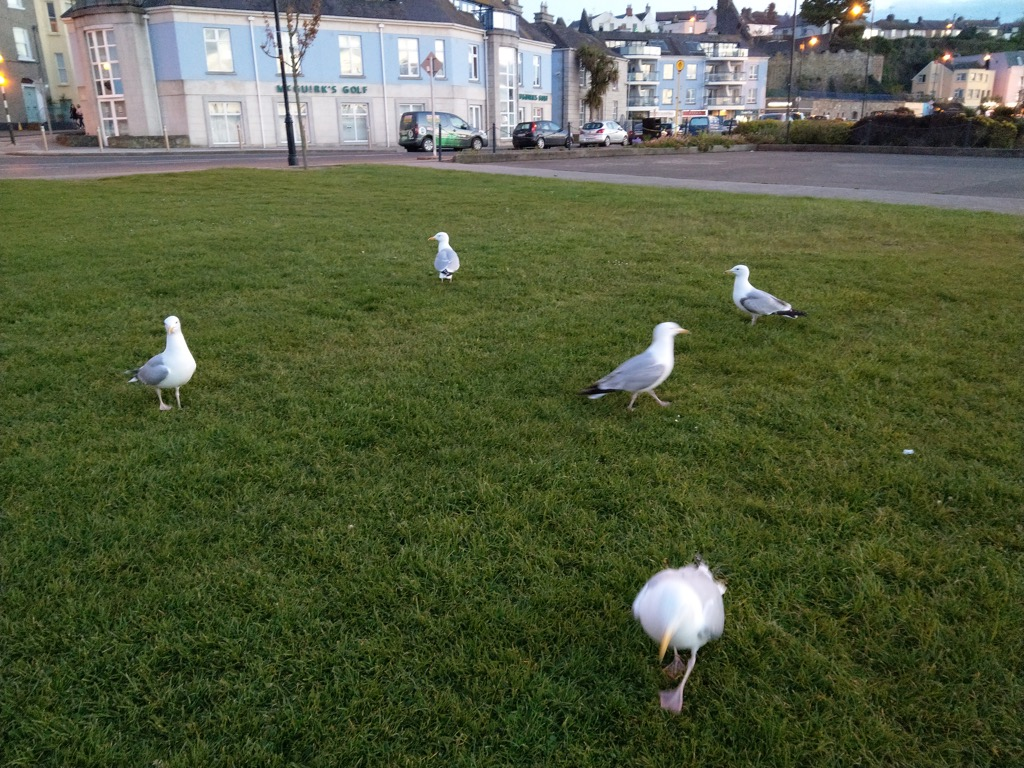
\includegraphics[width=\textwidth]{Sections/4InitialWork/4_images_obj_run3/photo.jpg}
  \end{subfigure}
  \begin{subfigure}{0.3\textwidth}
  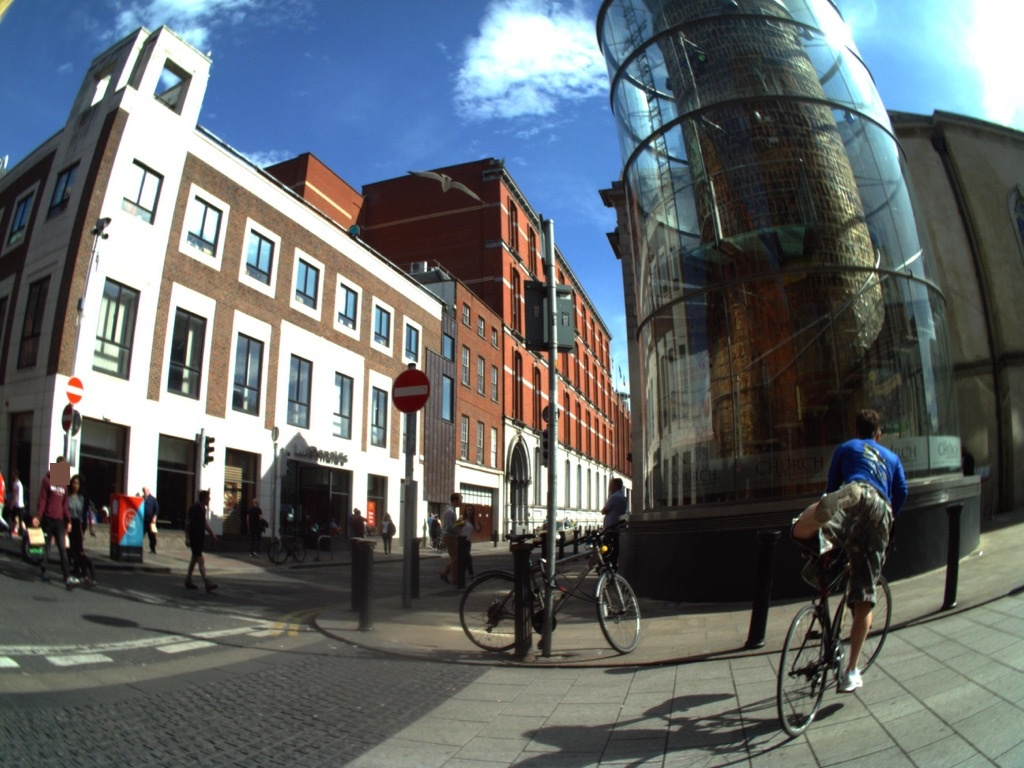
\includegraphics[width=\textwidth]{Sections/4InitialWork/4_images_obj_run4/photo.jpg}
  \end{subfigure}

  \caption{ 
  Pictures used for test runs.}
  \end{figure}

  \newpage
      \subsubsection{Object Detection Test Run Number 1}

    

      \begin{figure}[H]
        \centering
        \captionsetup{justification=centering}

        \begin{subfigure}{0.29\textwidth}
        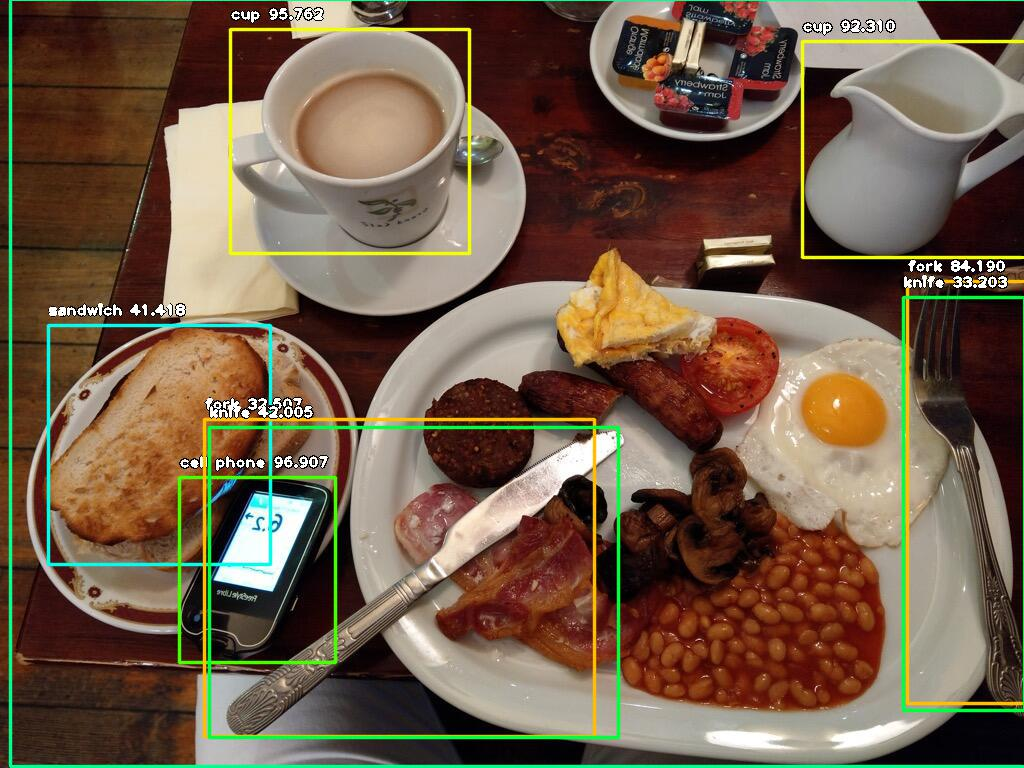
\includegraphics[width=\textwidth]{Sections/4InitialWork/4_images_obj_run1/retinaNet.jpg} 
        \caption{}
        \end{subfigure}
        \begin{subfigure}{0.65\textwidth}
        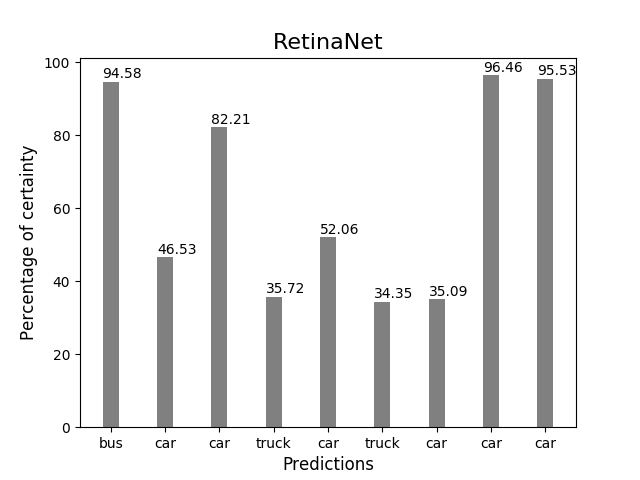
\includegraphics[width=\textwidth]{Sections/4InitialWork/4_images_obj_run1/retinaNet_graph.png}
        \caption{}
        \end{subfigure}
        
        \caption{ 
        Test run 1 with RetinaNet; a) Analysed picture with detections; b) Achieved performance on detections. }
        \end{figure}
    

      
        \begin{figure}[H]
          \centering
          \captionsetup{justification=centering}
  
          \begin{subfigure}{0.29\textwidth}
          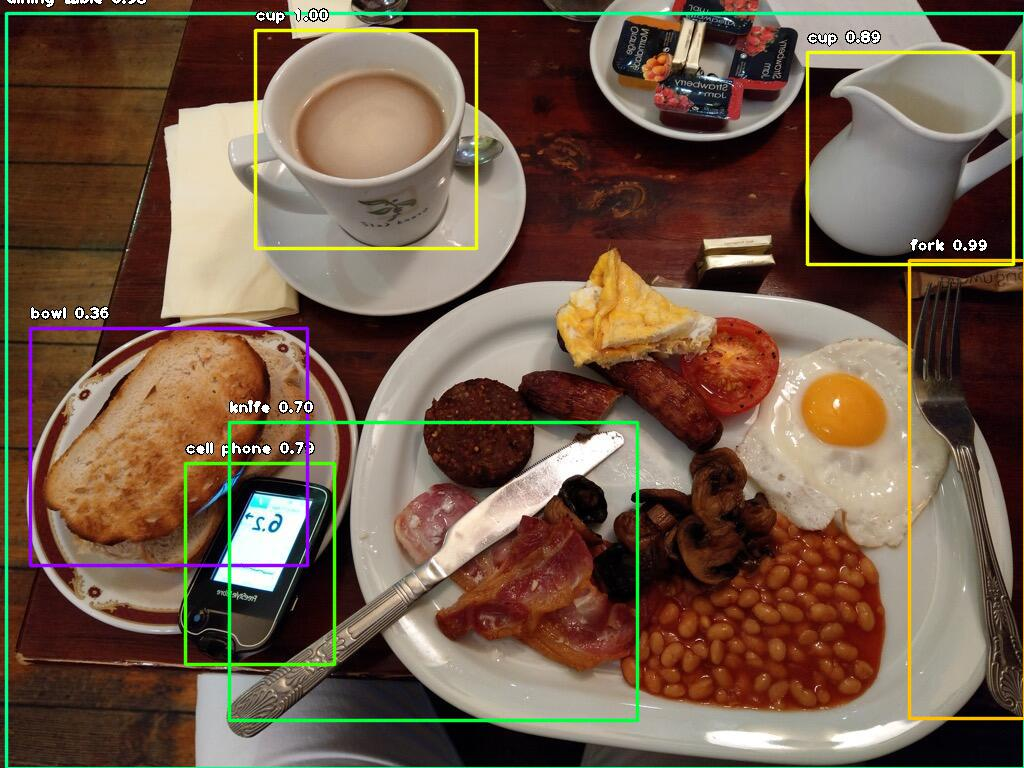
\includegraphics[width=\textwidth]{Sections/4InitialWork/4_images_obj_run1/yolo.jpg} 
          \caption{}
          \end{subfigure}
          \begin{subfigure}{0.65\textwidth}
          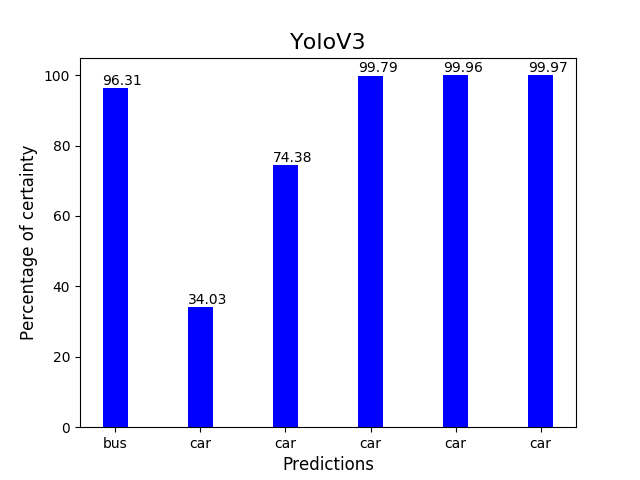
\includegraphics[width=\textwidth]{Sections/4InitialWork/4_images_obj_run1/yolo_graph.png}
          \caption{}
          \end{subfigure}
          
          \caption{ 
          Test run 1 with YOLOv3; a) Analysed picture with detections; b) Achieved performance on detections. }
          \end{figure}
      


          \begin{figure}[H]
            \centering
            \captionsetup{justification=centering}
    
            \begin{subfigure}{0.29\textwidth}
            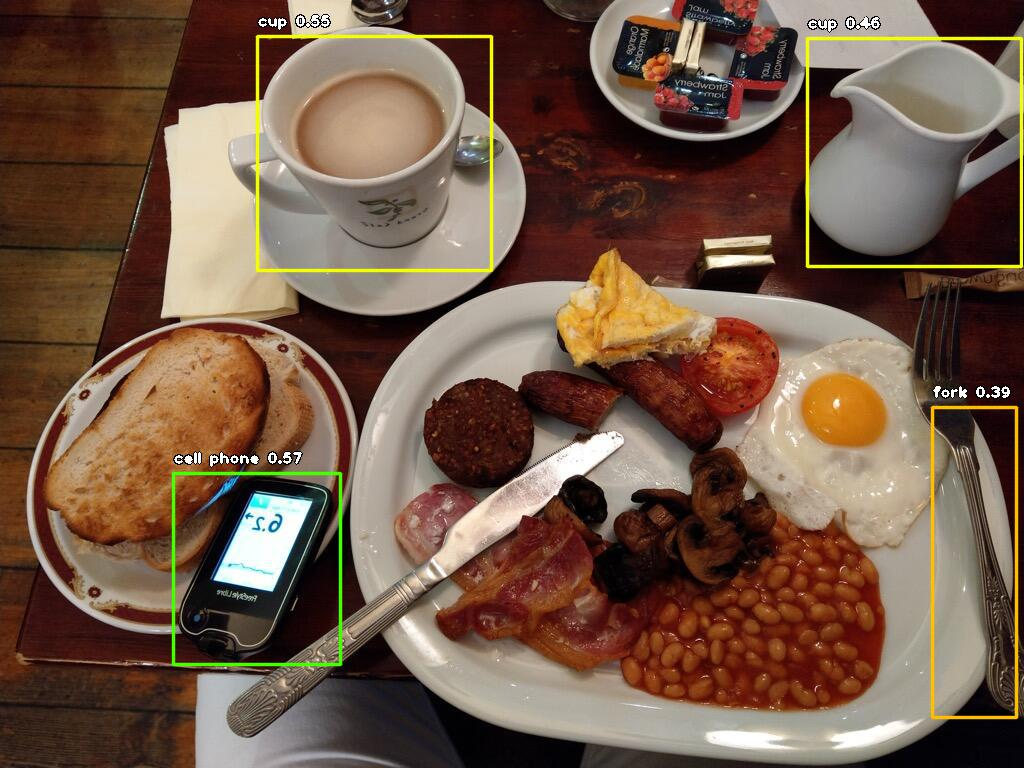
\includegraphics[width=\textwidth]{Sections/4InitialWork/4_images_obj_run1/yolo_tiny.jpg} 
            \caption{}
            \end{subfigure}
            \begin{subfigure}{0.4\textwidth}
            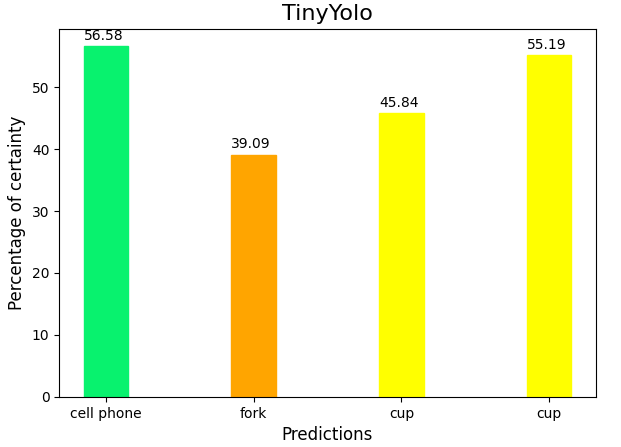
\includegraphics[width=\textwidth]{Sections/4InitialWork/4_images_obj_run1/tiny_yolo_graph.png}
            \caption{}
            \end{subfigure}
            
            \caption{ 
            Test run 1 with TinyYolo; a) Analysed picture with detections; b) Achieved performance on detections. }
            \end{figure}

      \newpage

  %%%%%%%%%%%%%%%%%%%%%%%%%%%%%%%%%%%%% run2   %%%%%%%%%%%%%%%%%%%%%%%%%%%%%%%%%%%%%
      
      \subsubsection{Object Detection Test Run Number 2}

  
    

      \begin{figure}[H]
        \centering
        \captionsetup{justification=centering}

        \begin{subfigure}{0.29\textwidth}
        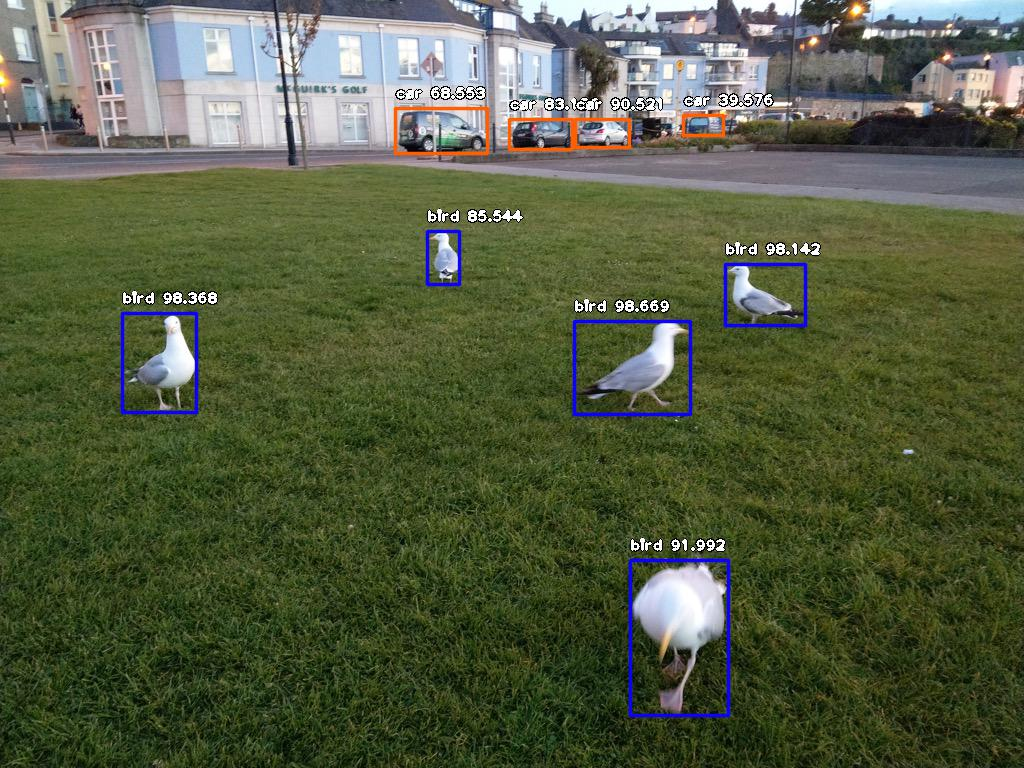
\includegraphics[width=\textwidth]{Sections/4InitialWork/4_images_obj_run3/retinaNet.jpg} 
        \caption{}
        \end{subfigure}
        \begin{subfigure}{0.65\textwidth}
        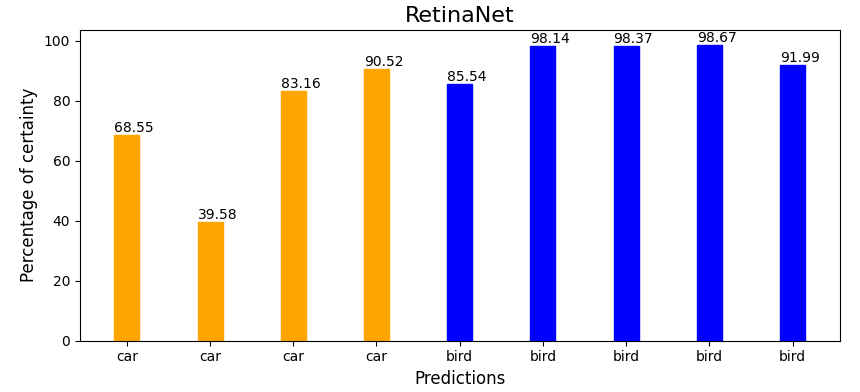
\includegraphics[width=\textwidth]{Sections/4InitialWork/4_images_obj_run3/retinaNet_graph.png}
        \caption{}
        \end{subfigure}
        
        \caption{ 
        Test run 2 with RetinaNet; a) Analysed picture with detections; b) Achieved performance detections. }
        \end{figure}



        \begin{figure}[H]
          \centering
          \captionsetup{justification=centering}
  
          \begin{subfigure}{0.29\textwidth}
          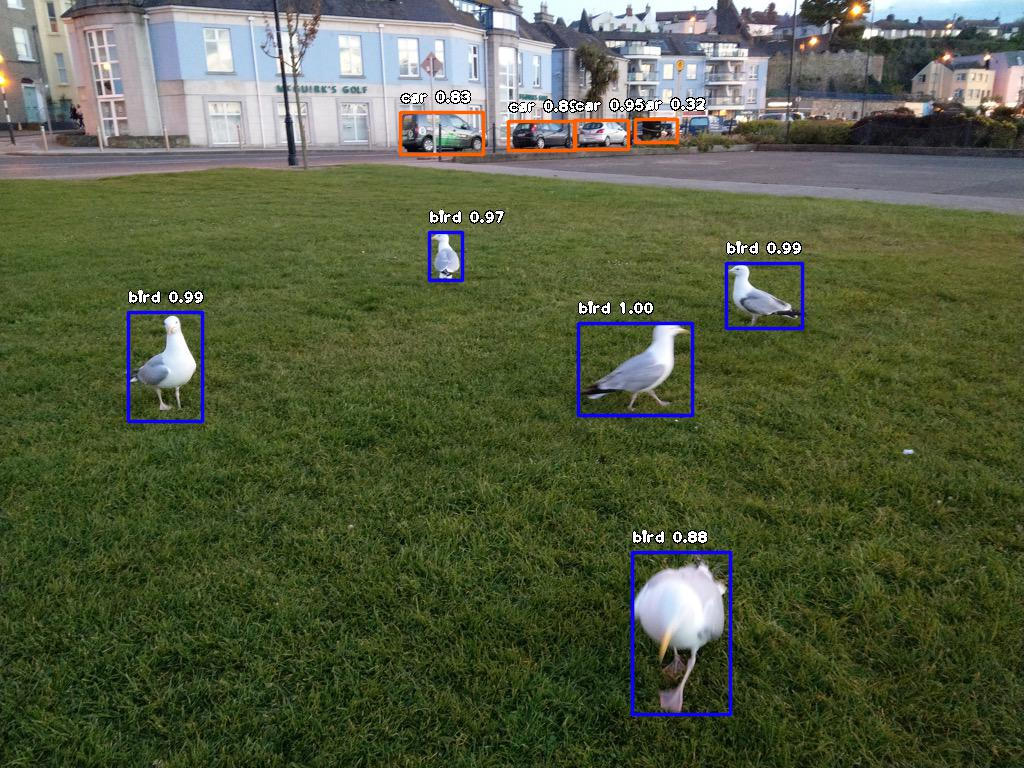
\includegraphics[width=\textwidth]{Sections/4InitialWork/4_images_obj_run3/yolo.jpg} 
          \caption{}
          \end{subfigure}
          \begin{subfigure}{0.65\textwidth}
          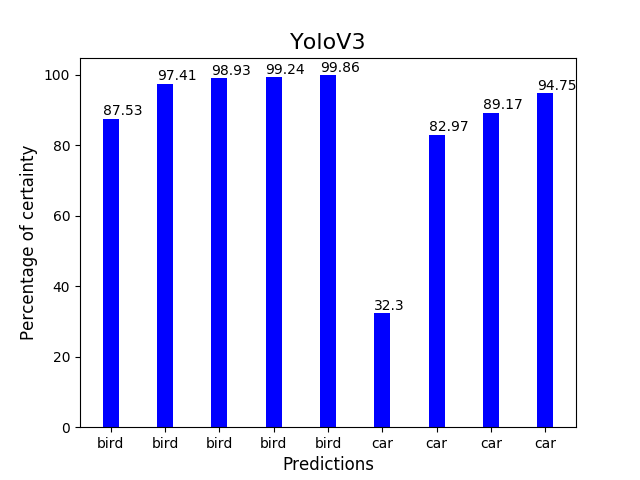
\includegraphics[width=\textwidth]{Sections/4InitialWork/4_images_obj_run3/yolo_graph.png}
          \caption{}
          \end{subfigure}
          
          \caption{ 
          Test run 2 with YoloV3 model; a) Analysed picture with detections; b) Achieved performance on detections. }
          \end{figure}
  

          \begin{figure}[H]
            \centering
            \captionsetup{justification=centering}
    
            \begin{subfigure}{0.29\textwidth}
            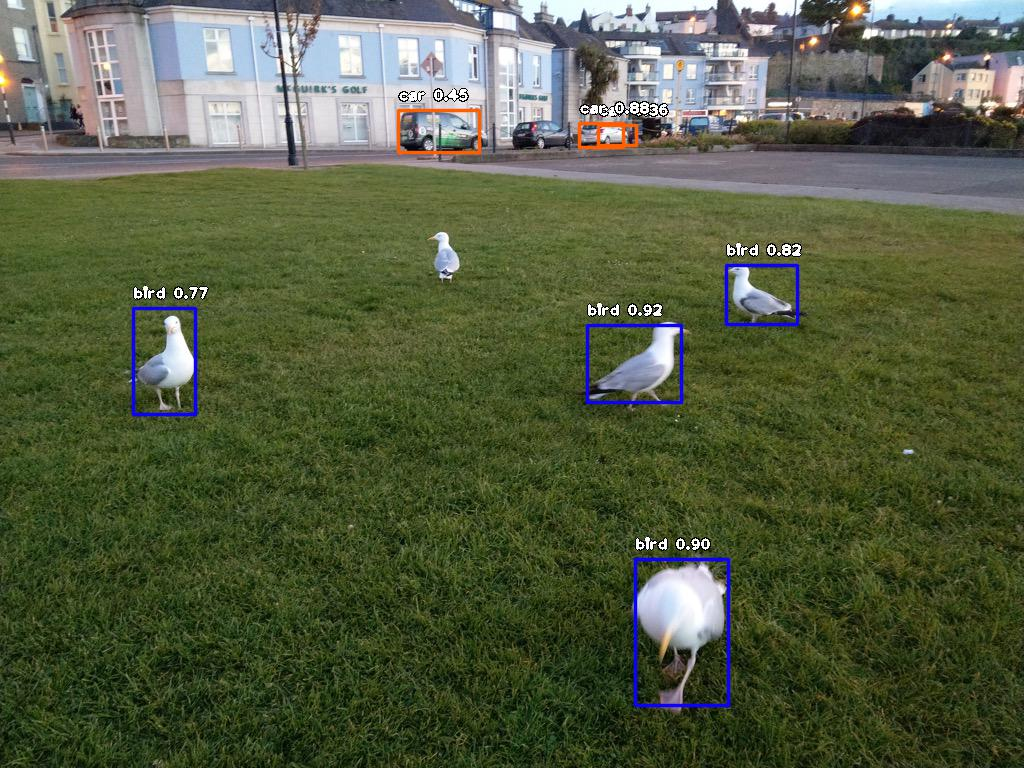
\includegraphics[width=\textwidth]{Sections/4InitialWork/4_images_obj_run3/yolo_tiny.jpg} 
            \caption{}
            \end{subfigure}
            \begin{subfigure}{0.6\textwidth}
            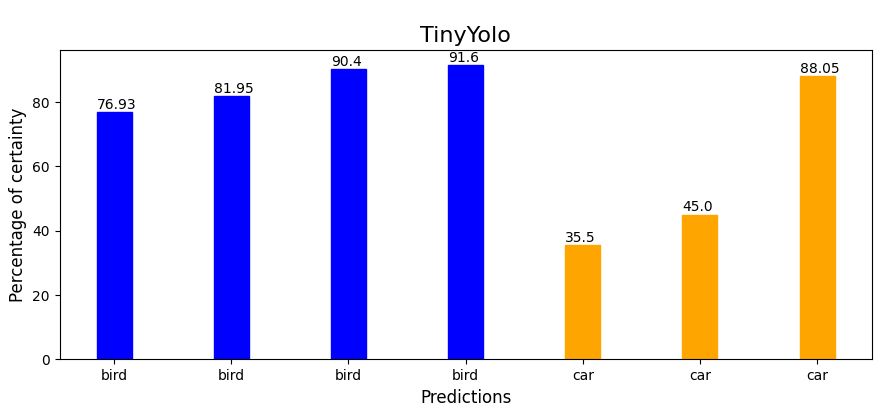
\includegraphics[width=\textwidth]{Sections/4InitialWork/4_images_obj_run3/yolo_tiny_graph.png}
            \caption{}
            \end{subfigure}
            
            \caption{ 
            Test run 2 with TinyYolo; a) Analysed picture with detections; b) Achieved performance on detections. }
            \end{figure}

      \newpage

      \subsubsection{Object Detection Test Run Number 3}



      \begin{figure}[H]
        \centering
        \captionsetup{justification=centering}

        \begin{subfigure}{0.29\textwidth}
        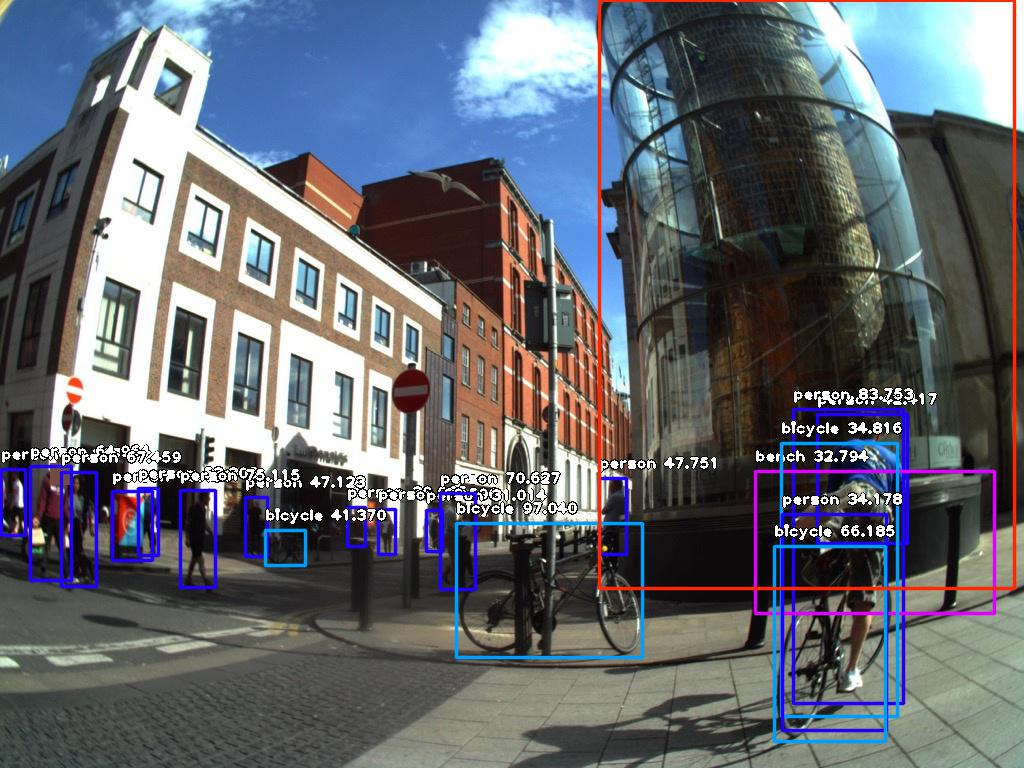
\includegraphics[width=\textwidth]{Sections/4InitialWork/4_images_obj_run4/retinaNet.jpg} 
        \caption{}
        \end{subfigure}
        \begin{subfigure}{0.7\textwidth}
        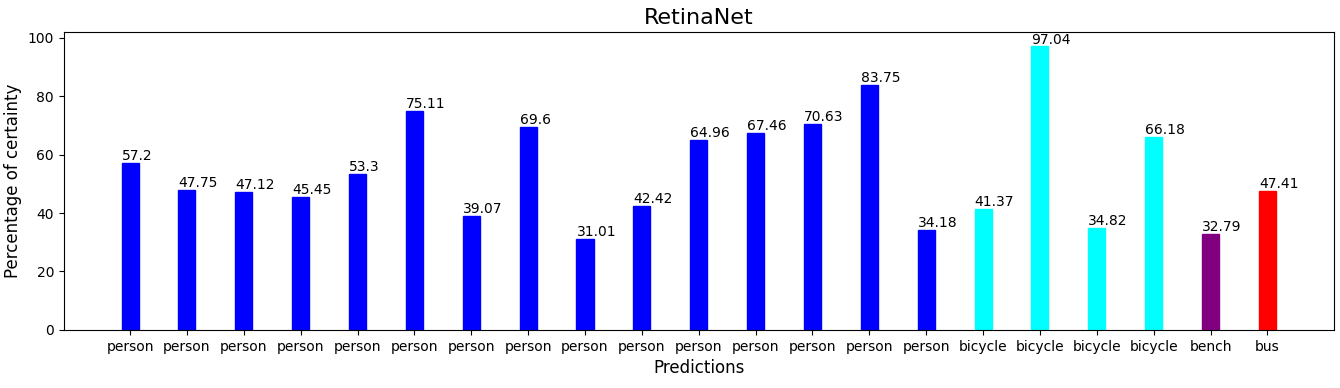
\includegraphics[width=\textwidth]{Sections/4InitialWork/4_images_obj_run4/retinaNet_graph.png}
        \caption{}
        \end{subfigure}
        
        \caption{ 
        Test run 3 with RetinaNet; a) Analysed picture with detections; b) Achieved performance detections. }
        \end{figure}



        \begin{figure}[H]
          \centering
          \captionsetup{justification=centering}
  
          \begin{subfigure}{0.29\textwidth}
          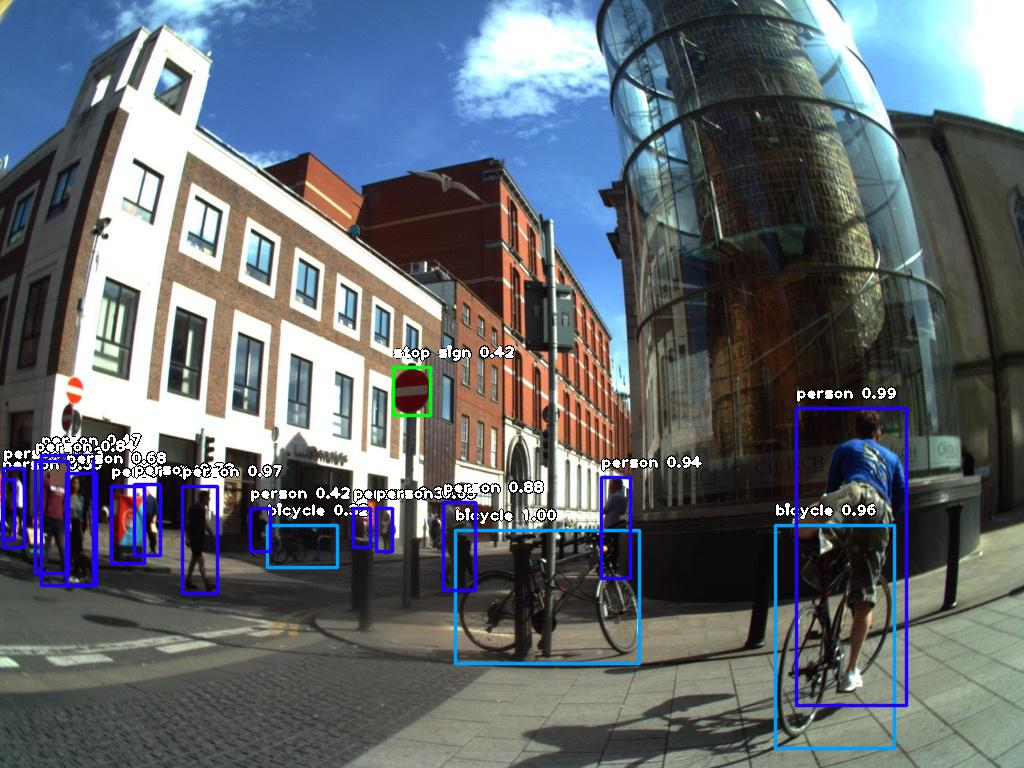
\includegraphics[width=\textwidth]{Sections/4InitialWork/4_images_obj_run4/yolo.jpg} 
          \caption{}
          \end{subfigure}
          \begin{subfigure}{0.7\textwidth}
          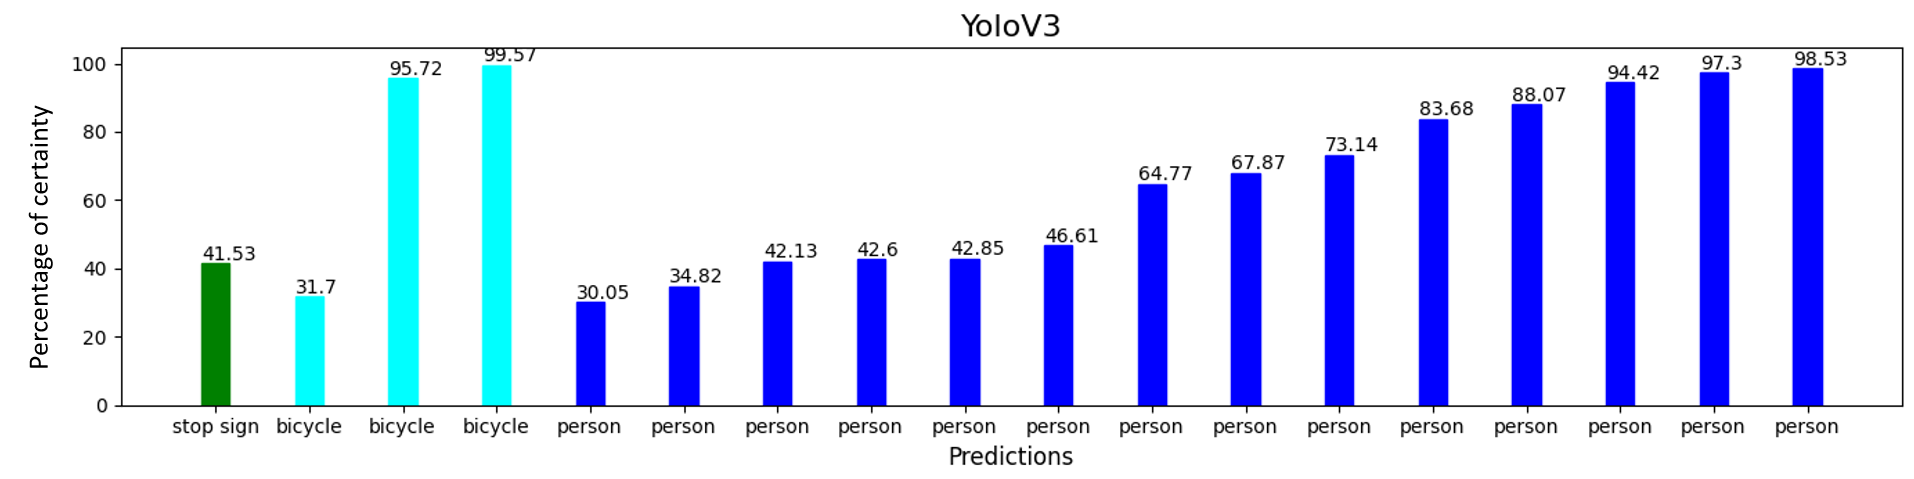
\includegraphics[width=\textwidth]{Sections/4InitialWork/4_images_obj_run4/yolo_graph.png}
          \caption{}
          \end{subfigure}
          
          \caption{ 
          Test run 3 with YoloV3 model; a) Analysed picture with detections; b) Achieved performance on detections. }
          \end{figure}
  

          \begin{figure}[H]
            \centering
            \captionsetup{justification=centering}
    
            \begin{subfigure}{0.29\textwidth}
            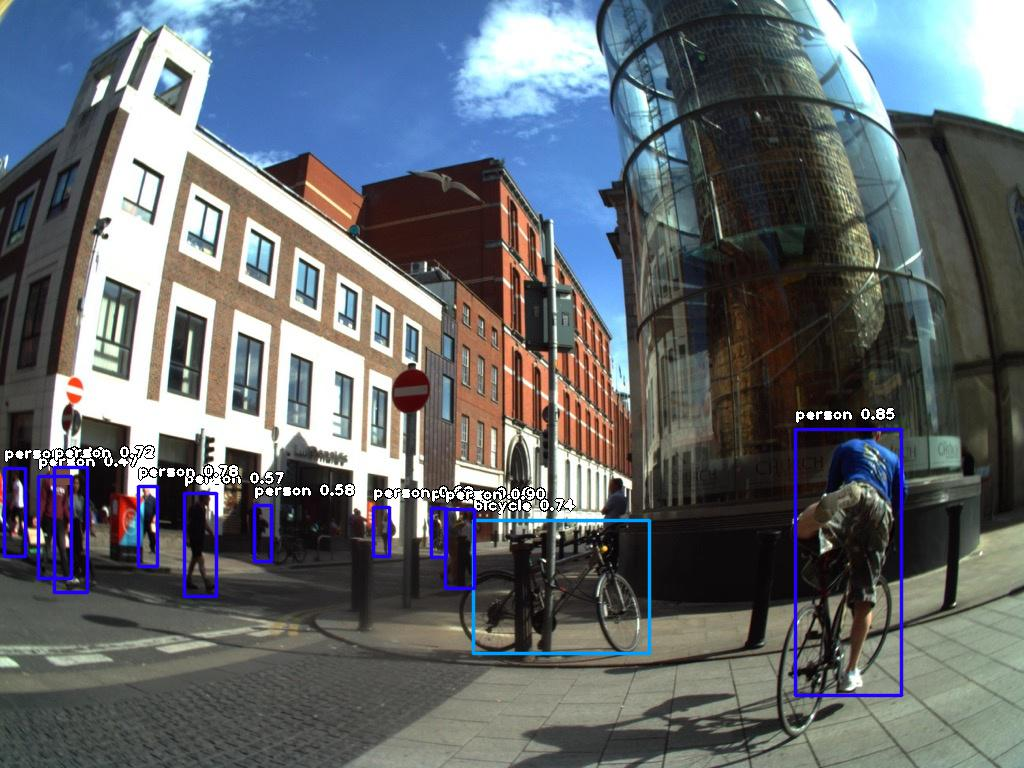
\includegraphics[width=\textwidth]{Sections/4InitialWork/4_images_obj_run4/yolo_tiny.jpg} 
            \caption{}
            \end{subfigure}
            \begin{subfigure}{0.65\textwidth}
            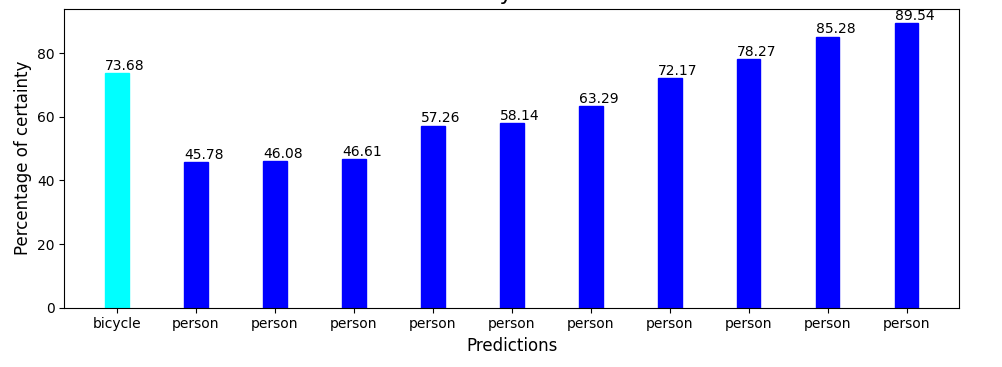
\includegraphics[width=\textwidth]{Sections/4InitialWork/4_images_obj_run4/tiny_yolo_graph.png}
            \caption{}
            \end{subfigure}
            
            \caption{ 
            Test run 3 with TinyYolo; a) Analysed picture with detections; b) Achieved performance on detections. }
            \end{figure}


    \newpage

    \subsection{Object Detection Word Clouds Generation Test Run}
    In order to make the labels extraction more easily visible and still achieve some degree of performance comparison between the 3 object detection models word clouds were generated.

    For this test 6 previously chosen images with identical setting were processed in order to generate 1 word cloud with all the extracted labels.
    
    In a word cloud, the bigger a word is the more times that label was detected in the pictures.


    \begin{figure}[H]
      \begin{subfigure}{\linewidth}
      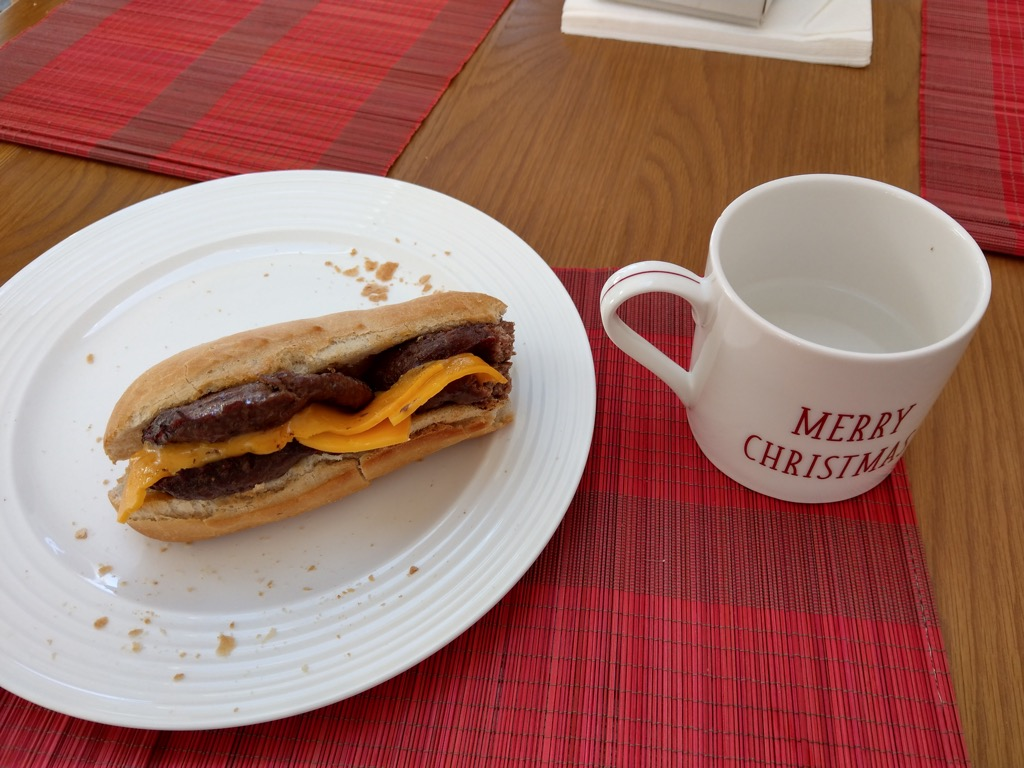
\includegraphics[width=.3\linewidth]{Sections/4InitialWork/4_images_wordcloud/photo1.jpg}\hfill
      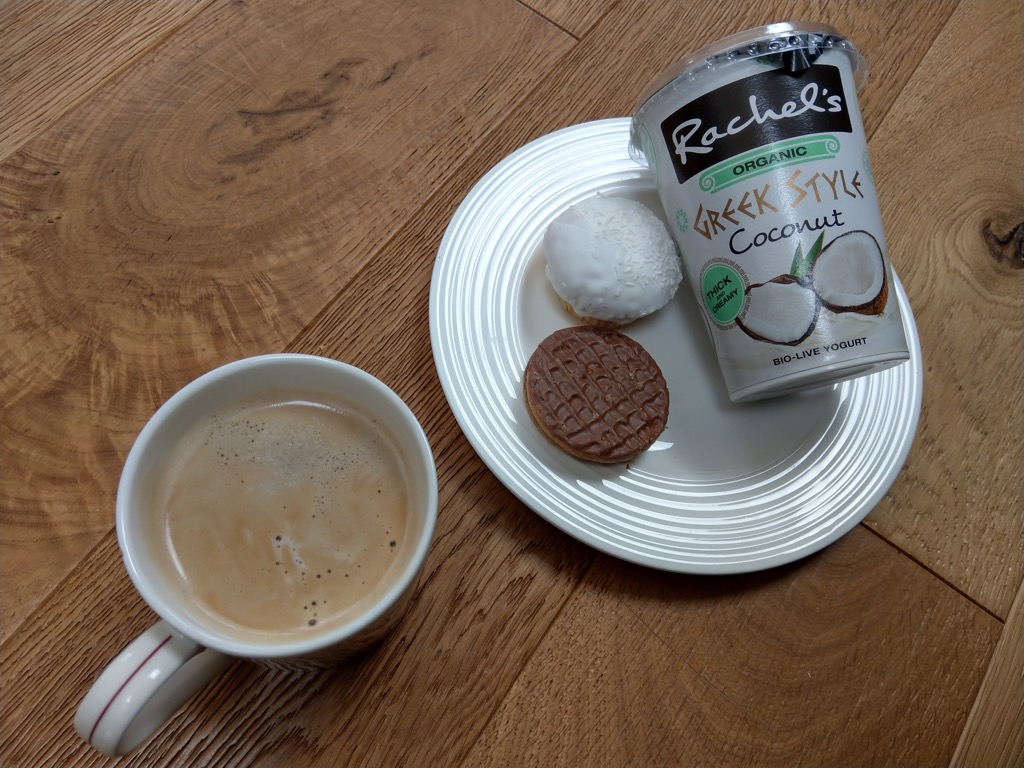
\includegraphics[width=.3\linewidth]{Sections/4InitialWork/4_images_wordcloud/photo2.jpg}\hfill
      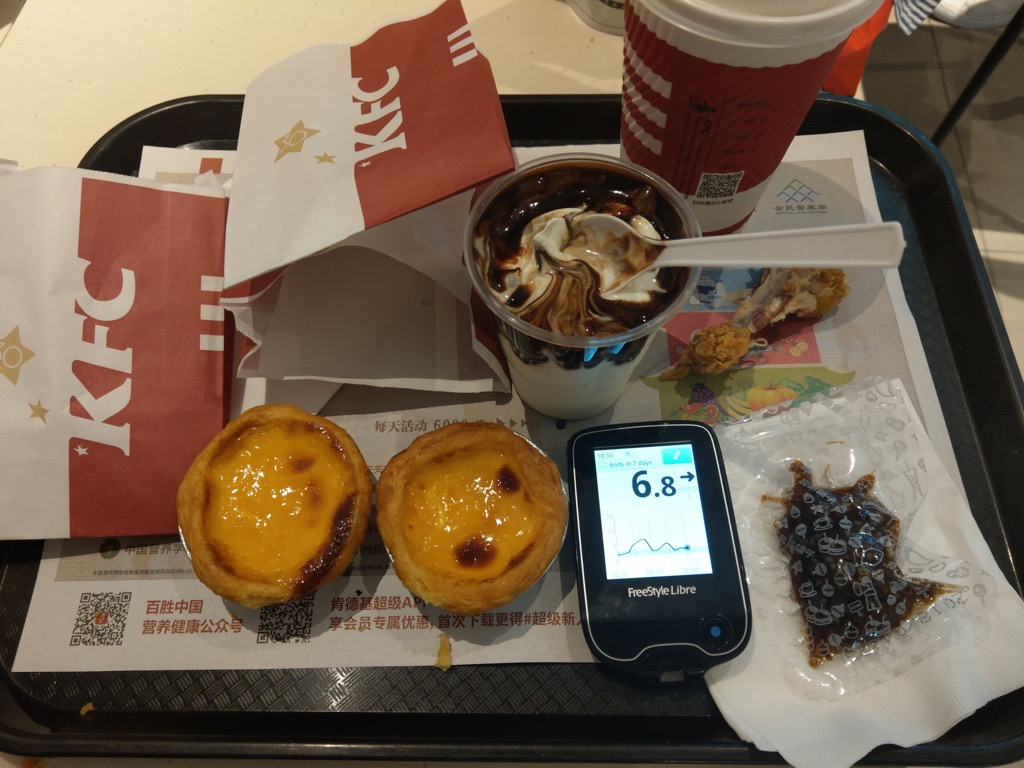
\includegraphics[width=.3\linewidth]{Sections/4InitialWork/4_images_wordcloud/photo7.jpg}
      \end{subfigure}\par\medskip
      \begin{subfigure}{\linewidth}
      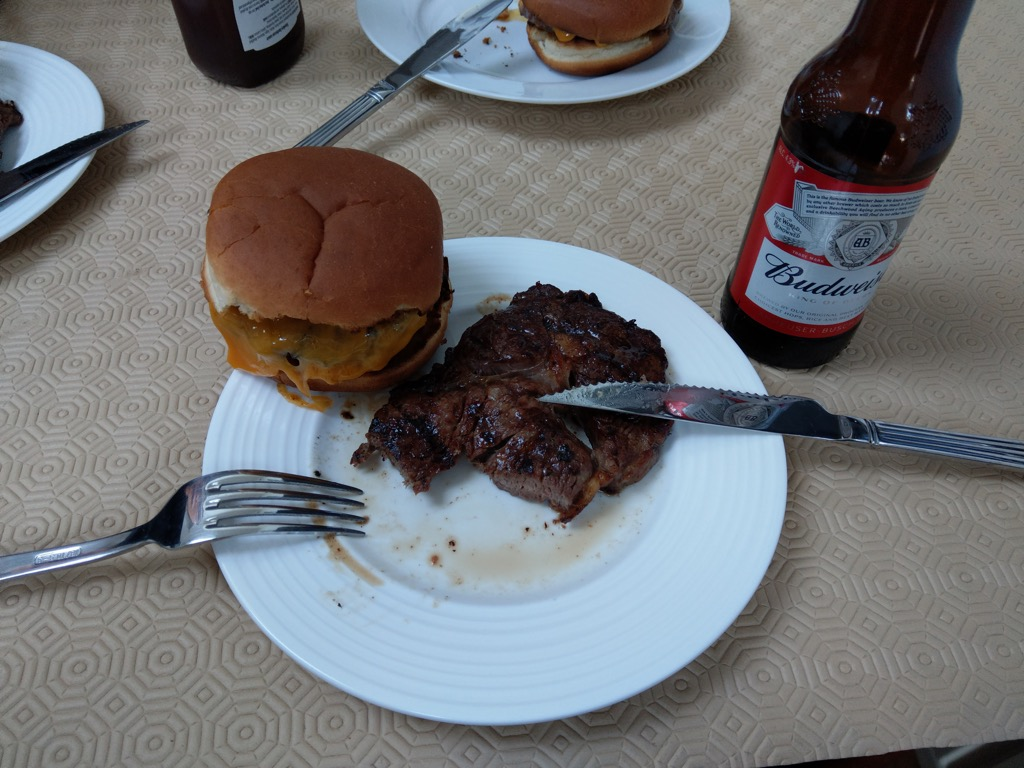
\includegraphics[width=.3\linewidth]{Sections/4InitialWork/4_images_wordcloud/photo4.jpg}\hfill
      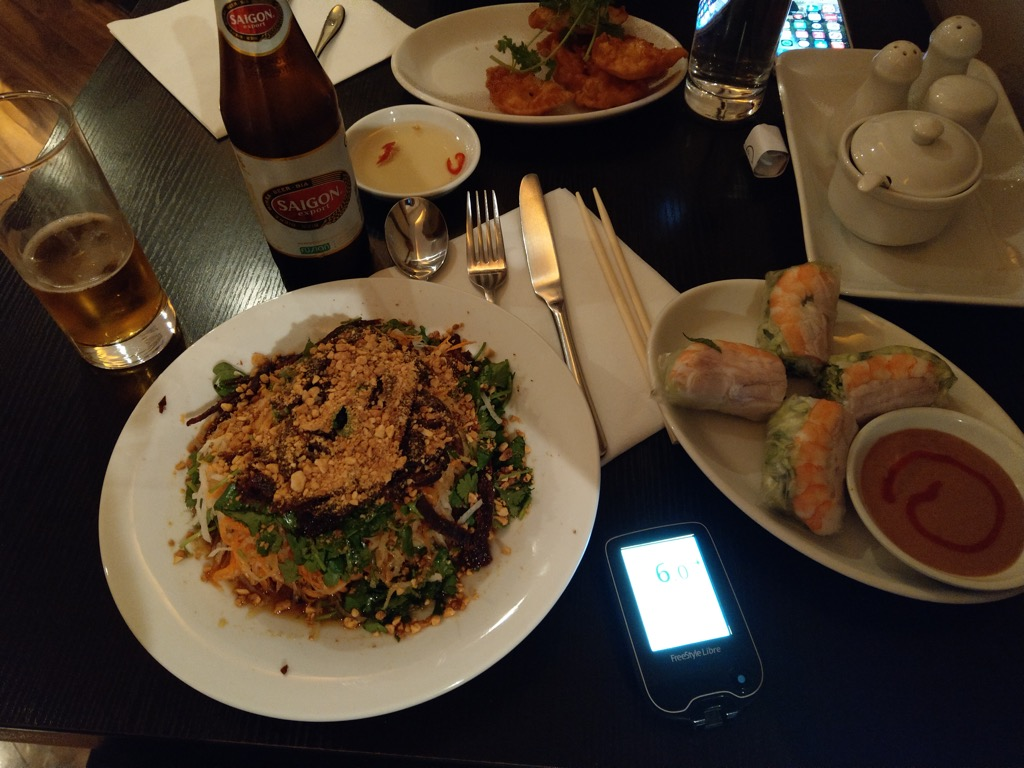
\includegraphics[width=.3\linewidth]{Sections/4InitialWork/4_images_wordcloud/photo5.jpg}\hfill
      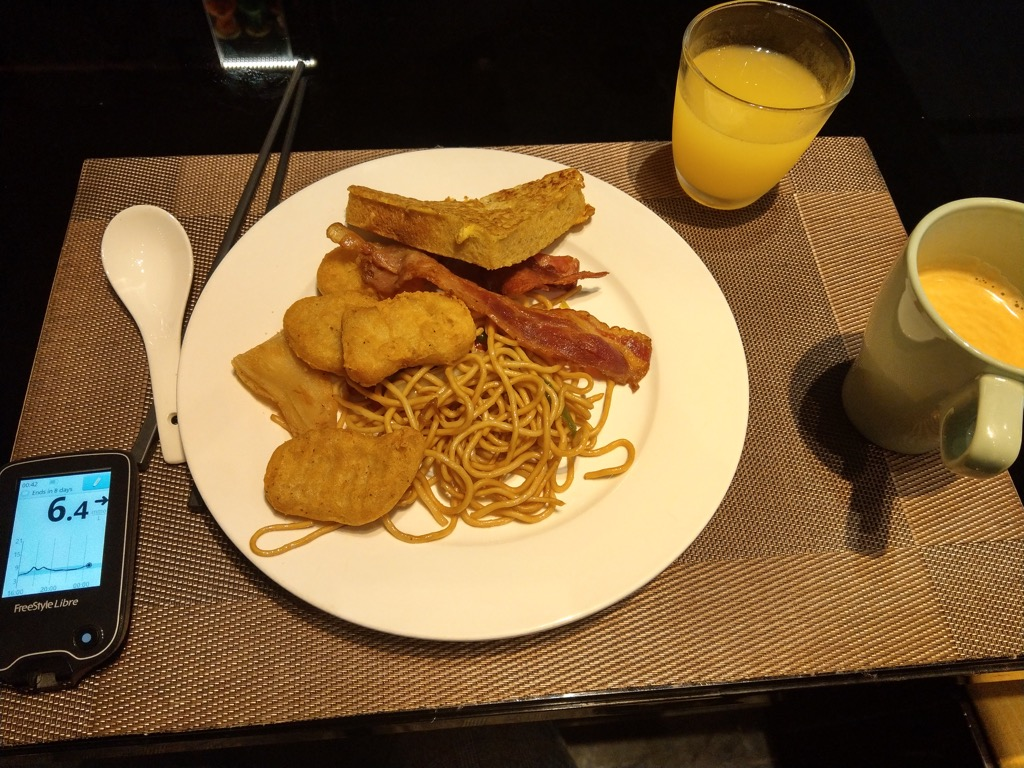
\includegraphics[width=.3\linewidth]{Sections/4InitialWork/4_images_wordcloud/photo6.jpg}
      \end{subfigure}\par\medskip
      \caption{Used images for word cloud generation.}
    \end{figure}



    \subsubsection{Word Clouds}

    \begin{figure}[H]
      \centering
      \captionsetup{justification=centering}
    
      \begin{subfigure}{0.33\textwidth}
      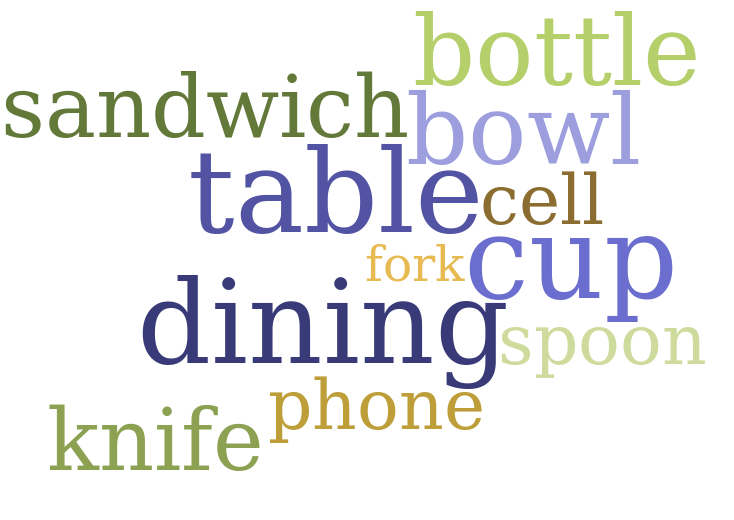
\includegraphics[width=\textwidth]{Sections/4InitialWork/4_images_wordcloud/yolo_pic.png} 
      \caption{}
      \end{subfigure}
      \begin{subfigure}{0.33\textwidth}
      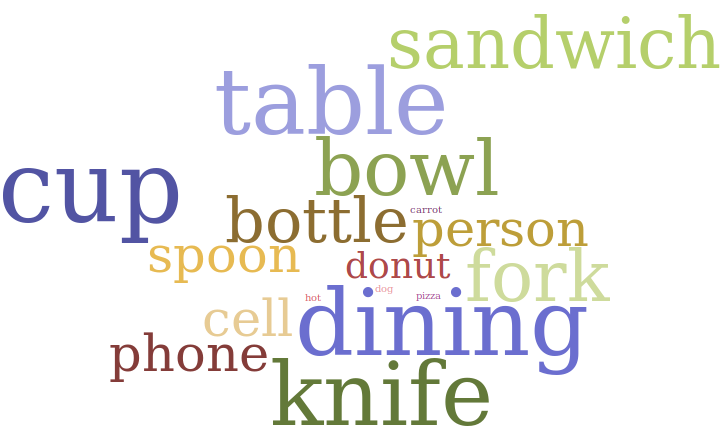
\includegraphics[width=\textwidth]{Sections/4InitialWork/4_images_wordcloud/retina_pic.png}\hfill
      \caption{}
      \end{subfigure}
      \begin{subfigure}{0.3\textwidth}
      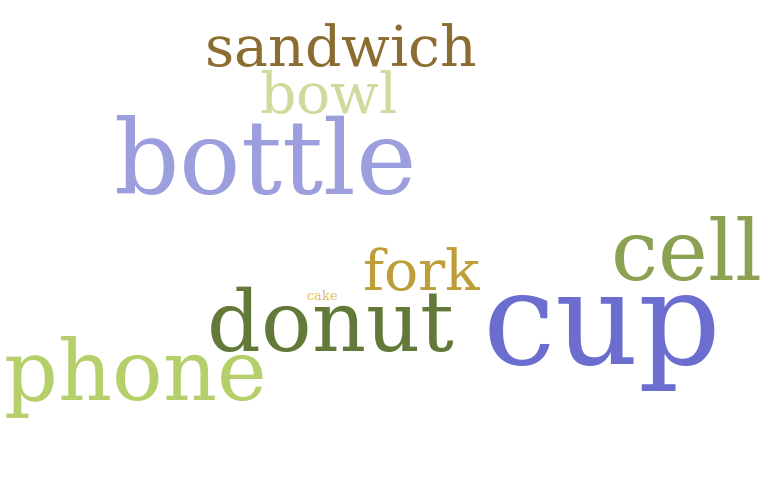
\includegraphics[width=\textwidth]{Sections/4InitialWork/4_images_wordcloud/tiny_yolo_pic.png}\hfill
      \caption{}
      \end{subfigure}
      \caption{Generated Word Clouds; a) Yolo word cloud; b) RetinaNet word cloud; c) TinyYolo word cloud}
    \end{figure}

    \newpage
    

    \subsubsection{Object Detection Results Analysis}
      \label{sec:results_objet}


     From the different test runs it is possible to analyse that the TinyYolo model under performs severely compared to RetinaNet and YoloV3. This is expected, as explained in section \ref{sec:tiny_yolo} the TinyYolo model is a smaller model of YOLOv3 that requires less computational resources and that is better suited for more constrained environments with smaller targets.

     Comparing RetinaNet to YoloV3 it is possible to conclude that YoloV3 is more accurate than RetinaNet. For example in the first run, RetinaNet detects knifes and forks in the same place, in third example RetinaNet detects a bus in the place of a building while Yolo is capable of detecting a correctly stop sign that no other model detected.

     As for the word clouds, it is possible to notice that in the YoloV3 cloud and the retinaNet cloud there are many more words than the tinyyolo cloud, again, tinyyolo is severely under performing when compared to the other 2 model.
     
     Looking at the Yolo model word cloud its possible to notice some consistency because most of the words have the same size. In the RetinaNet word cloud there are many words from different sizes, this can occur because RetinaNet wrongly detects 1 or 2 object like "pizza", "donut and "person" in one of the images.

     This test runs allow for the conclusion that the YoloV3 model is the better performing one, and therefore was the one chosen for the object detections for the automatic retrieval system. However, since the interactive system was built with detections from ResNeXt-101, those detections were also reutilized for the automatic system in a different run for the imageclef challenge. This will be further discussed in section \ref{sec:runs}.


\section{Example of a Raw Retrieval System}
\label{sec:alpha_retrieval}

As a first step in building a fully automatic retrieval system an "alpha system" was created without any text processing and very raw on the way it worked. Simply put, a user just needs to write a label, according to one of the words available for detection, and the system will scan all the images that are inside a directory and return the images that have detections of that specific user inputted label. The user is also able to input the minimum percentage probability for the detections, therefore, if the user chooses "cup" and "40\%", objects that are not "cup" or that are "cup" but below the threshold of 40\% wont be returned.

\begin{figure}[H]
  \centering
  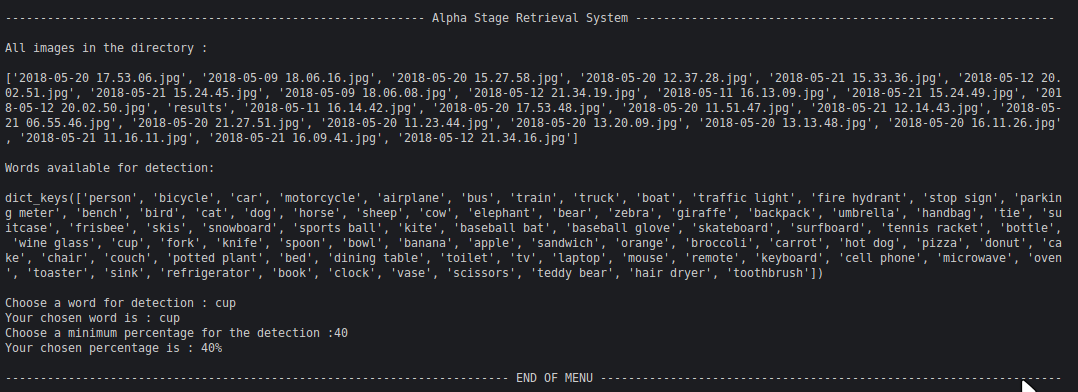
\includegraphics[width = \textwidth]{Sections/4InitialWork/4_images_random/alpha.png}
  \caption{System capable of detecting specific user inputted labels in multiple images. }
  \label{fig:yolov3} 
\end{figure}




\begin{figure}[H]
  \begin{subfigure}{\linewidth}
  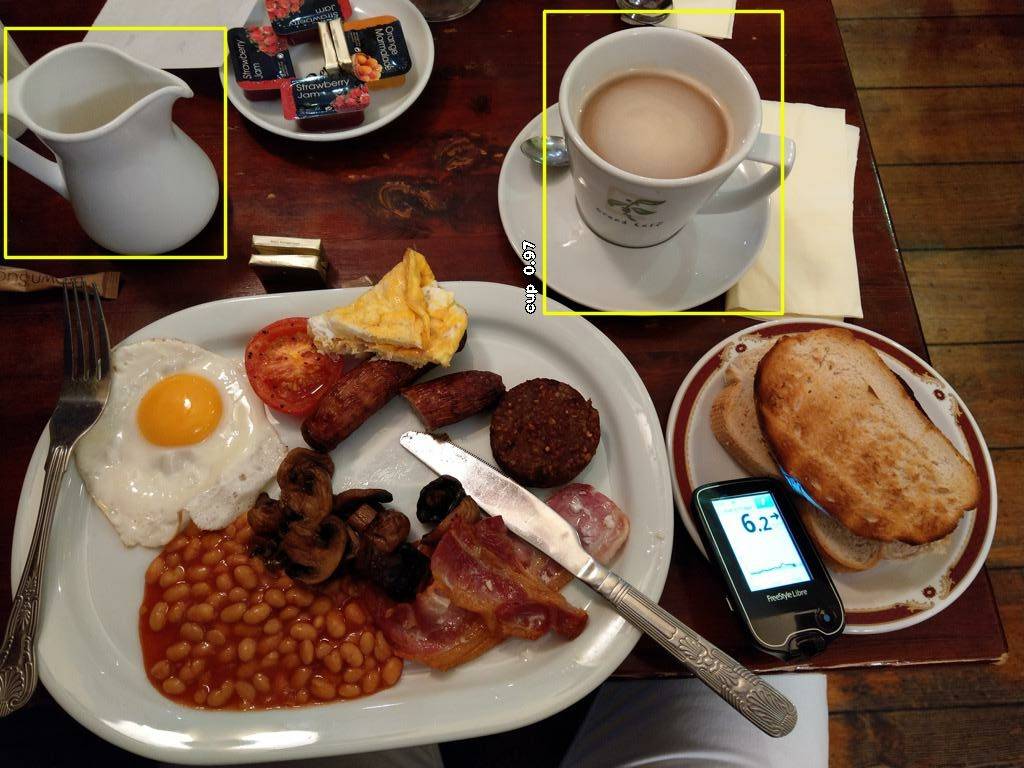
\includegraphics[width=.3\linewidth]{Sections/4InitialWork/4_images_alphasystem/alpha_yolo_2.jpg}\hfill
  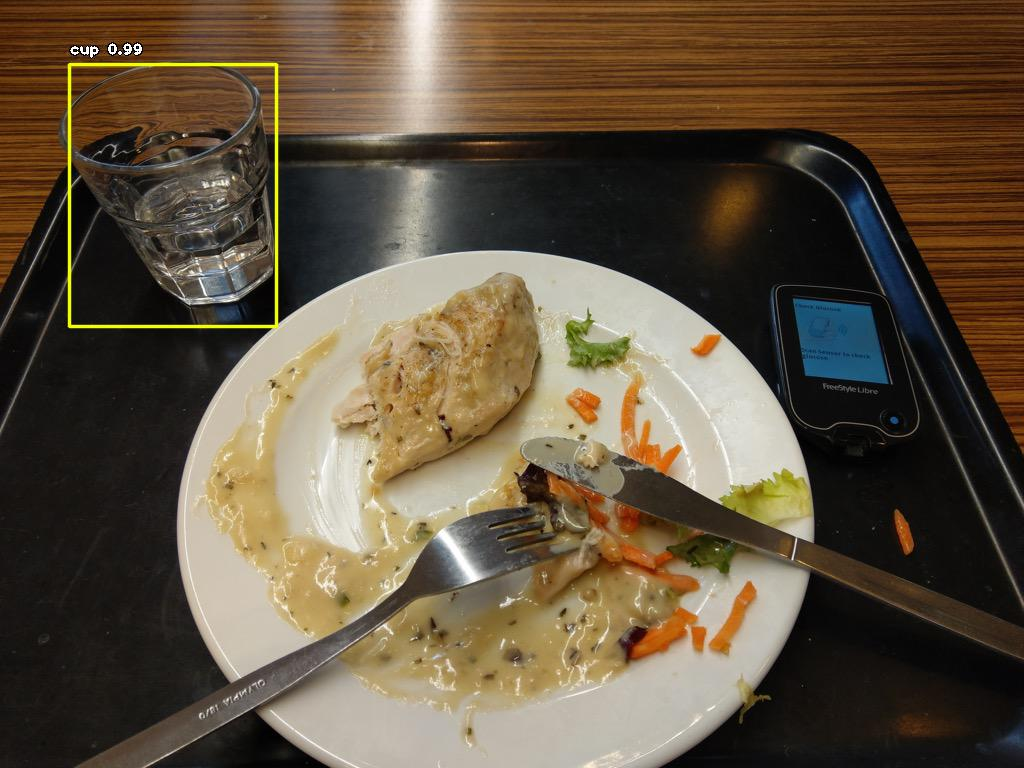
\includegraphics[width=.3\linewidth]{Sections/4InitialWork/4_images_alphasystem/alpha_yolo_3.jpg}\hfill
  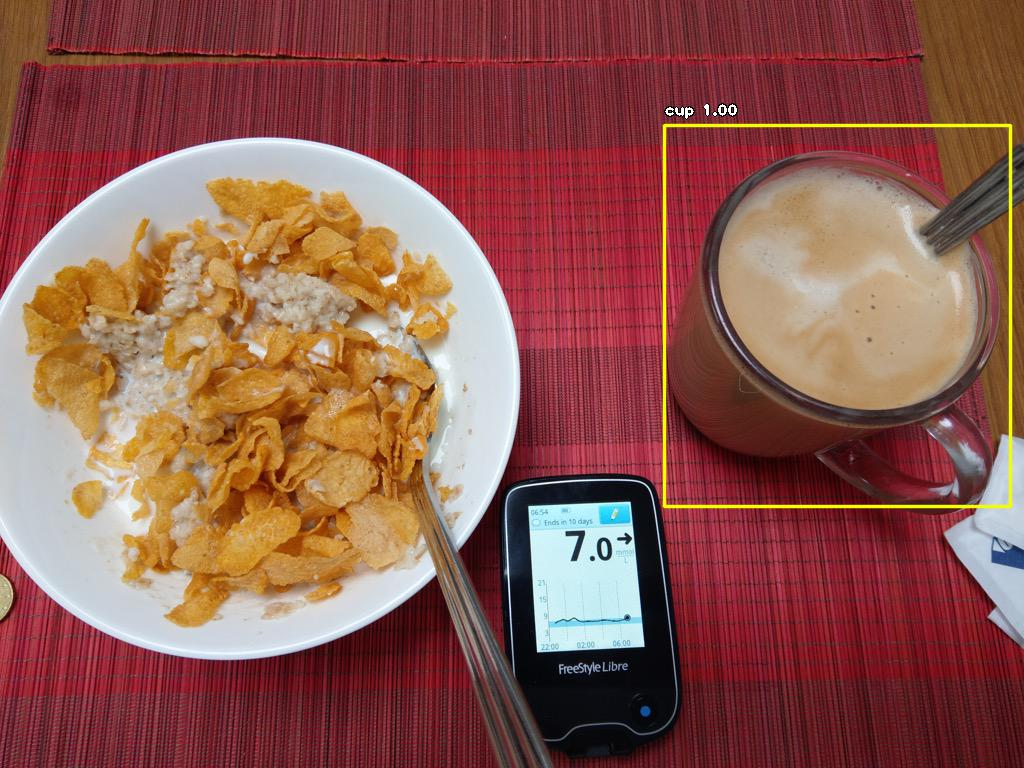
\includegraphics[width=.3\linewidth]{Sections/4InitialWork/4_images_alphasystem/alpha_yolo_4.jpg}
  \end{subfigure}\par\medskip
  \begin{subfigure}{\linewidth}
  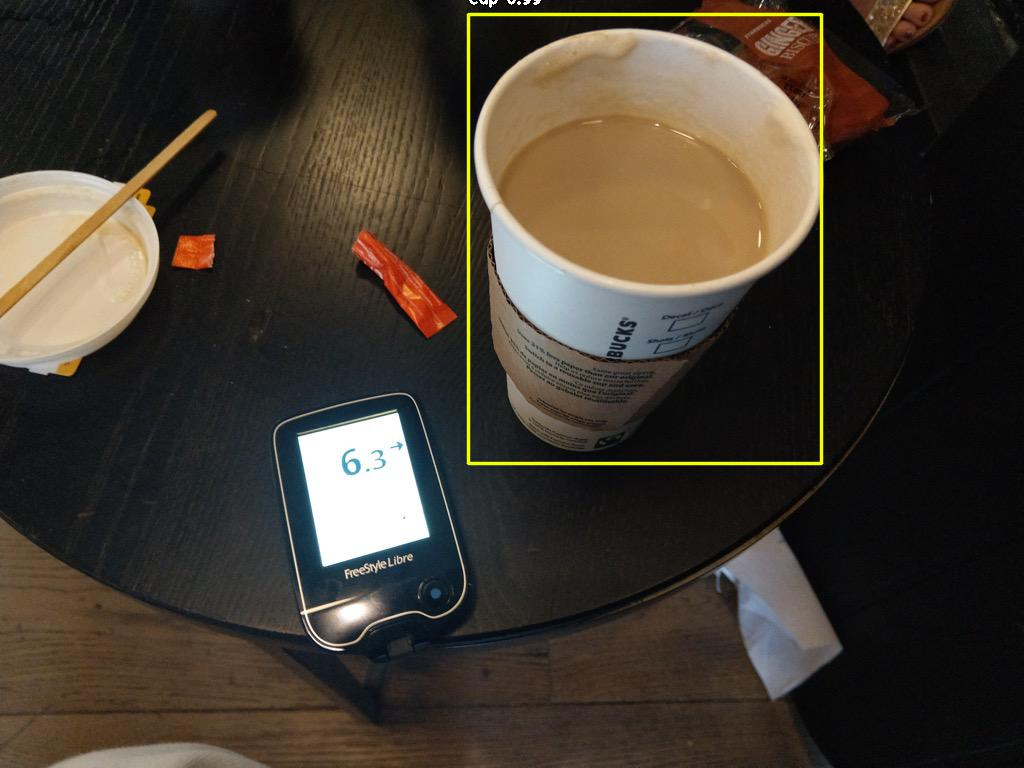
\includegraphics[width=.3\linewidth]{Sections/4InitialWork/4_images_alphasystem/alpha_yolo_5.jpg}\hfill
  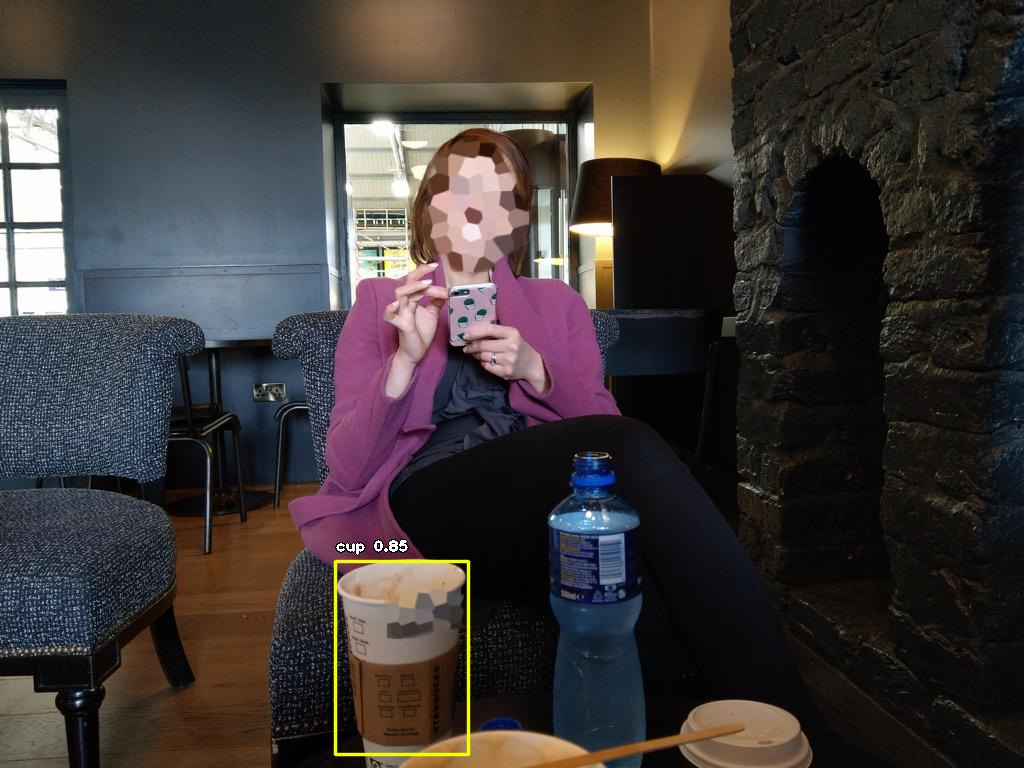
\includegraphics[width=.3\linewidth]{Sections/4InitialWork/4_images_alphasystem/alpha_yolo_6.jpg}\hfill
  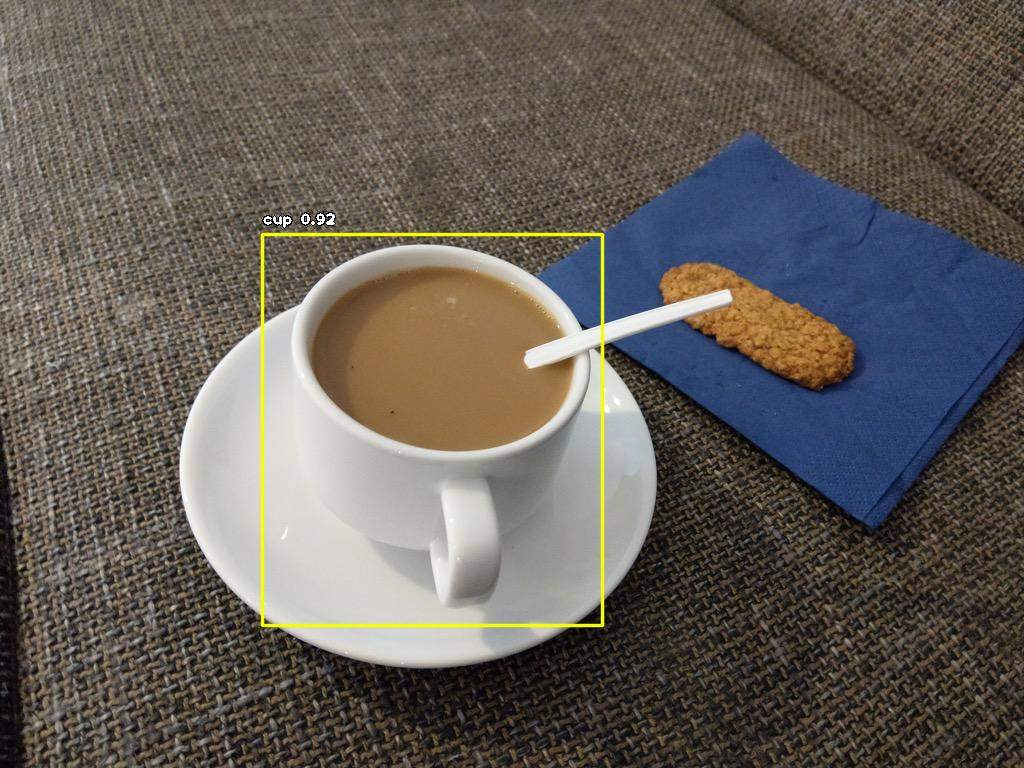
\includegraphics[width=.3\linewidth]{Sections/4InitialWork/4_images_alphasystem/alpha_yolo_7.jpg}
  \end{subfigure}
  \caption{Retrieved images for the label "cup" with "40\%" threshold.}
\end{figure}

\section{Scene Recognition}
\label{sec:scene_recognition}
  In order to detect interiors, exteriors and places a pretrained model provided by Zhou et al. \cite{Zhou2018}  trained on the Places365 standard dataset was used .

  The following example shows the extractions done to a random image from the imageclef dataset. 

  \begin{figure}[H]
    \centering
    \captionsetup{justification=centering}

    \begin{subfigure}{0.525\textwidth}
    
    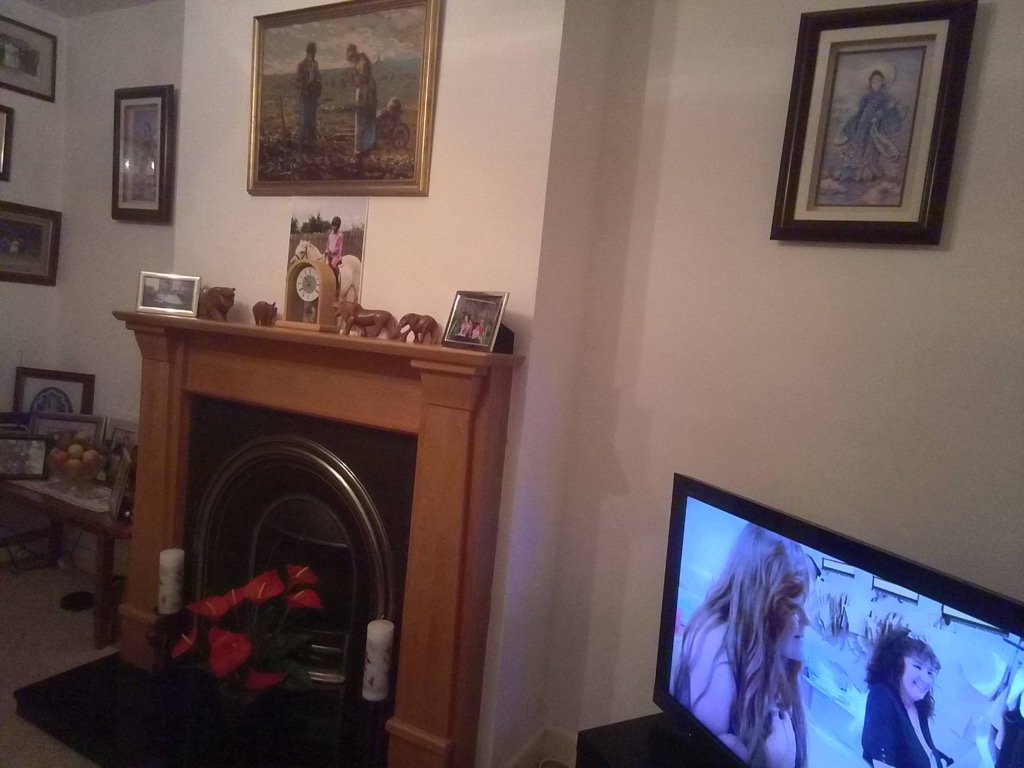
\includegraphics[width=\textwidth]{Sections/4InitialWork/4_images_random/dataset_place.jpg} 
    \caption{}
    \end{subfigure}
    \begin{subfigure}{0.4\textwidth}
    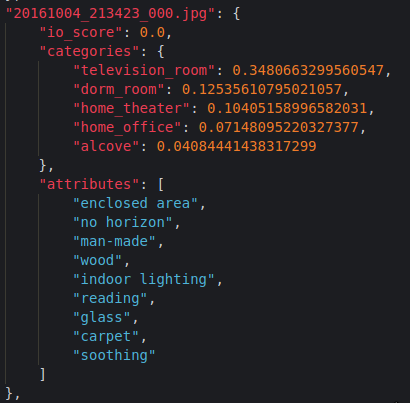
\includegraphics[width=\textwidth]{Sections/4InitialWork/4_images_random/places_detect.png}
    \caption{}
    \end{subfigure}
    
    \caption{Example of a scene recognition; a) Picture 20161004\_213423\_000.jpg from the imageclef dataset; b) Scene recognition model output for that image.}

    \label{fig:imagea}
    \end{figure}


    The "io\_score" represents the interior vs exterior certainty. It ranges from 0 to 1. If its close to 0 it means the image is probably an interior and if it is close to 1 it means it is probably an exterior. In this example, the image is an interior and the "io\_score" is 0, therefore the model predicted correctly that the image is in fact an interior.

    Following up, the "categories" is where the model tries to predict what the image represents in terms of a scene. In this case the model predicts with 34.8\% accuracy that it is a "television\_room" which is also correct, since the image represents a division of a house with a television.

    Finally, the "attributes" is the section where the model tries to describe the picture. Some of the predicaments were "enclosed area", "man-made", "indoor lightning" and so on which are all correct since the image represents a man-made enclosed space structure with indoor-lightning.

\section{Run  1 and Run 2}
\label{sec:runs}
    In this year challenge, 2 different runs were made with the automatic retrieval system. 
    
    For the first run the extract objects from the images is a combination of ResNeXt-101 and Feature Pyramid Network architectures in a basic Faster Region-based Convolutional Network (Faster R-CNN) pretrained on the COCO dataset that was proposed by Mahajan et al. \cite{Mahajan2018}
    
    In the second run, the object detection algorithm used is the YoloV3 \cite{Redmon2018} model pretrained in the COCO dataset. 

    This was done in order to understand if different object detection algorithms, would help in achieving better results.

\section{Processing the Imageclef Dataset}
\label{sec:process_dataset}

    In order to extract the maximum possible labels, all images in the imageclef dataset were fully processed with YOLOv3 or with ResNeXt-101 and the Places scene recognition model. This is an exhaustive approach since it takes a lot of computer processing time and resources. 
    
    Using \ref{fig:imagea} a) as an example, the fully processed image looks like this:
    
    \begin{figure}[H]
      \centering
      \captionsetup{justification=centering}
  
      \begin{subfigure}{0.395\textwidth}
      
      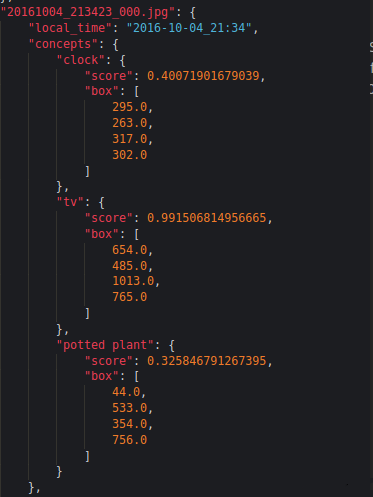
\includegraphics[width=\textwidth]{Sections/4InitialWork/4_images_random/process1.png} 
      \end{subfigure}
      \begin{subfigure}{0.49\textwidth}
      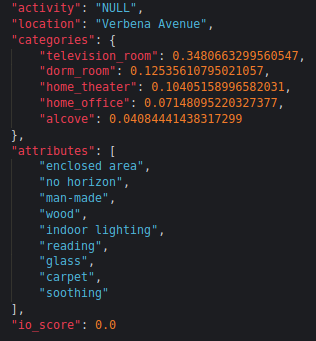
\includegraphics[width=\textwidth]{Sections/4InitialWork/4_images_random/process2.png}
      \end{subfigure}
      \caption{Fully processed image with YOLOv3 and PLACES365.}
      \label{fig:image_fully_processed}
      \end{figure}


       
    \begin{figure}[H]
      \centering
      \captionsetup{justification=centering}
  
      \begin{subfigure}{0.3\textwidth}
      
      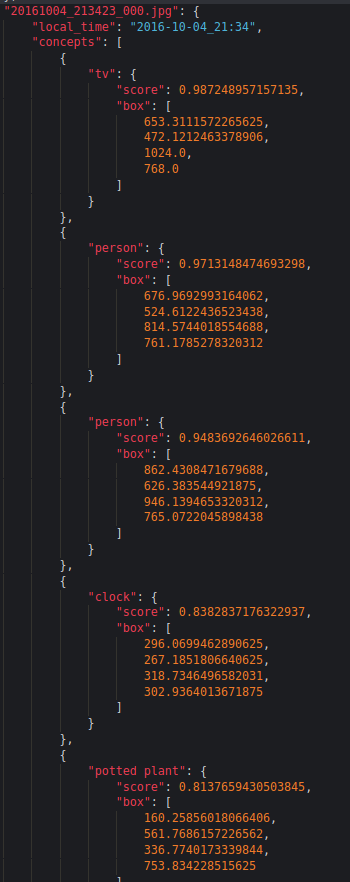
\includegraphics[width=\textwidth]{Sections/4InitialWork/4_images_random/res1.png} 
      \end{subfigure}
      \begin{subfigure}{0.3\textwidth}
      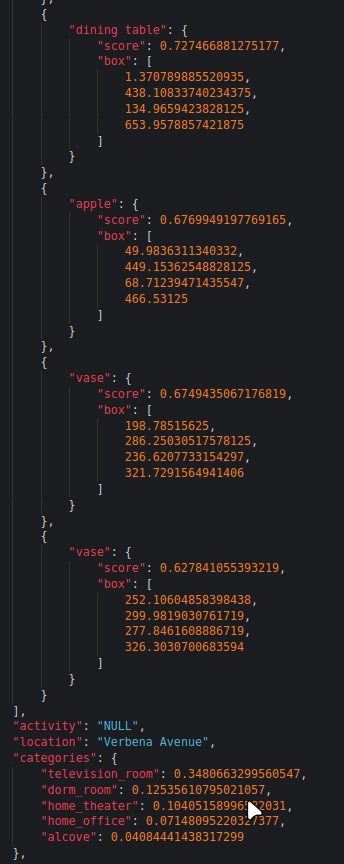
\includegraphics[width=\textwidth]{Sections/4InitialWork/4_images_random/res2.png}
      \end{subfigure}
      \begin{subfigure}{0.3\textwidth}
        \includegraphics[width=\textwidth]{Sections/4InitialWork/4_images_random/res3.png}
        \end{subfigure}
      \caption{Fully processed image with ResNeXt-101 and PLACES365.}
      \label{fig:image_fully_processed_resnext}
      \end{figure}


      The "activity" and "location" were extracted from the data provided by the organizers in a .csv file. Unfortunately that data is not accurate enough, and a good option would be to use activity recognition algorithms to extract activities from images. unfortunately the processing time was already to high with the current setup.
      The "local\_time" was extracted directly from the picture name.
      The "box" is the location of the given "concept" in the image according to the pixels of the image.


